% ===========================================================================
% III. STRUCTURAL VERIFIABILITY OF NEURAL NETWORKS
% ===========================================================================
\section{Structural Verifiability of Neural Networks}
\label{sec:svnn}

We now formalize a central observation that emerged from the compiler design
process: whether a neural network compiler can provide design-time correctness
guarantees is not solely a property of the compiler---it is fundamentally
determined by the \textit{architecture} being compiled. This section defines
the class of architectures for which correctness-preserving compilation is
achievable, proves that KAN belongs to this class, and demonstrates that
standard MLPs do not.

\vspace{4pt}
\begin{remark}[The Compilable Frontier]
\label{rem:compilable_frontier}
The SVNN conditions define a \textbf{compilable frontier}---a principled
boundary separating neural architectures whose deployed behavior can be
certified at design time from those that require runtime testing. Architectures
satisfying Conditions~1--2 lie on the \textit{interior} (certifiable side):
their decomposition into pure linear and element-wise operations enables the
structural induction that Theorem~2's proof relies on. Architectures violating
any condition lie on the \textit{exterior} (empirical-only side): they can
still be compiled and deployed, but their correctness guarantees are limited
to test-set validation. Proposition~1 (below) establishes that standard MLPs
with SiLU, Sigmoid, or Tanh activations---the dominant architectures in
industrial ML---lie on the exterior. This frontier is not an implementation
artifact; it reflects a fundamental property of which function classes admit
closed-form, compiler-computable error propagation.
\end{remark}


\subsection{The Verification Challenge for PLC-Deployed Networks}
\label{sec:svnn-challenge}

Industrial PLCs govern safety-critical machinery: conveyor sorting systems,
motor drives, and process control loops where incorrect outputs can cause
equipment damage or production line stoppage. Deploying neural networks on
such controllers therefore demands correctness guarantees that go beyond
empirical test-set accuracy.

Existing ML$\to$PLC tools (RTNNIgen~\cite{rtnnigen2024}, MLconverter%
~\cite{mlconverter2025}, ICSML~\cite{icsml2023}) provide \textit{no}
mathematical guarantee that the generated PLC code preserves the trained
model's behavior. Their correctness model is purely empirical: train, convert,
and test on a held-out set. For industrial deployment---where inputs may
drift, sensors may degrade, and the PLC's REAL arithmetic differs from
PyTorch's float32---this is insufficient.

We identify three levels of deployment verification, in increasing order
of strength:

\begin{enumerate}
    \item \textbf{Level 1---Runtime Testing (Weakest):} Evaluate the deployed
          model on a test set and report accuracy. This is the status quo
          (RTNNIgen, MLconverter). It provides no guarantee on unseen inputs
          and cannot detect systematic floating-point discrepancies.
    \item \textbf{Level 2---Design-Time Error Bounds (SVNN):} Compute, at
          \textit{compile time} and without executing on hardware, a provable
          per-output error bound $\varepsilon_i$ such that for all valid
          inputs $x$, the deployed model's output differs from the trained
          model's output by at most $\varepsilon_i$. This is the guarantee
          that \neuroplc provides (Theorem~1).
    \item \textbf{Level 3---Mechanized Formal Verification (Strongest):}
          A machine-checked proof (e.g., in Coq, Isabelle, or Lean) that the
          compiler preserves semantics down to the IEEE~754 bit-level. This
          has been achieved for select neural network kernels in TorchLean%
          \cite{torchlean2025} but is currently intractable for full
          compiler pipelines.
\end{enumerate}

Level~2---design-time error bounds---is the appropriate level for
industrial deployment. The question is: \textit{which architectures admit
such bounds, and why?}

\subsection{Definition: Structurally Verifiable Neural Network (SVNN)}
\label{sec:svnn-definition}

\begin{definition}[Structurally Verifiable Neural Network]
\label{def:svnn}
A neural network architecture $\mathcal{A}$ is \textbf{structurally
verifiable} (SVNN) with respect to a compiler $C$ if for any instance
$M \in \mathcal{A}$, the compiler can compute, at design time and without
executing $M$ on target hardware, a per-output error bound
$\varepsilon_i(M, X)$ such that:
\begin{equation}
\sup_{x \in X} \|M(x)_i - C(M)(x)_i\|_\infty \leq \varepsilon_i(M, X)
\quad \forall i \in \{1, \dots, d_{\text{out}}\}
\label{eq:svnn_def}
\end{equation}
where $X \subset \mathbb{R}^{d_{\text{in}}}$ is the validated input domain
and $C(M)$ denotes the compiler's generated code executing on the target
platform's arithmetic (here, IEC~61131-3 REAL $\equiv$ IEEE~754 binary32).
\end{definition}

This definition captures the essential requirement: the compiler must
provide an \textit{a priori} guarantee---before the model ever runs on the
PLC---that the deployed code will not silently diverge from the trained
model. The error bound $\varepsilon_i$ may depend on the model's parameters,
the compiler's approximation choices (e.g., LUT resolution), and the input
domain, but it must be computable from these quantities alone.

\subsection{Sufficient Conditions for SVNN}
\label{sec:svnn-conditions}

We now establish the architectural conditions that enable SVNN compilation.
The conditions formalize why some architectures admit tight, composable
error bounds while others do not.

\vspace{4pt}
\noindent\textbf{Theorem 2 (SVNN Sufficient Conditions).}
\label{thm:svnn_conditions}
Let $\mathcal{A}$ be a feedforward neural network architecture. If $\mathcal{A}$
satisfies Conditions~1 and~2 below, then $\mathcal{A}$ is structurally
verifiable---for any instance $M \in \mathcal{A}$ of finite depth $L$, a
compiler adhering to the SVNN compilation discipline can compute, from the
model parameters alone, a finite per-output error bound. If $\mathcal{A}$
additionally satisfies the contractivity refinement (Condition~3), this bound
admits the closed, \textit{depth-independent} geometric-series form
$O(M_{\max} \cdot h^2 \cdot d_{\max} / (1-\gamma))$, where $M_{\max}$ is the
maximum second-derivative bound, $h$ is the LUT grid spacing, $d_{\max}$ the
maximum activation count per layer, and $\gamma < 1$ the contractivity
constant; absent Condition~3, the bound remains finite for every fixed $L$
but may grow with depth.

The conditions are designed to \textit{discriminate}: a standard MLP layer
$\mathbf{h} = \sigma(W\mathbf{x} + \mathbf{b})$ composes an affine transform
and a pointwise activation in one coupled operation, violating Condition~1.
This prevents per-operation error induction (the proof's structural induction
requires each node to be either purely linear or purely element-wise).
MLPs with SiLU or GELU additionally violate the Z3-verifiability of
Condition~2 (the transcendental $\exp$ is undecidable in Z3's NRA theory);
MLPs with ReLU lack a $C^2$ curvature parameter. KAN layers, in contrast,
decompose naturally at the IR level into separate MatMul, BsplineLUT,
StandardAct, and Add nodes---each satisfies one of the two pure types.
Conditions~1--2 thus characterize exactly the class that admits the
induction, and KAN belongs to it; standard MLPs do not.

\begin{enumerate}
    \item \textbf{Operation-Type Closure (Condition~1).} The architecture
    can be decomposed into a directed acyclic graph where every node is
    either (a) a linear transformation (matrix multiplication, vector
    addition) or (b) an element-wise univariate function. No node may
    mix these operation types. This decomposition is provided by the
    compiler's IR ({\S}\ref{sec:ir}); it guarantees that the per-node
    error induction in the proof below never encounters a coupled
    linear+nonlinear operation.

    \item \textbf{Univariate Curvature Bound (Condition~2).} Every element-wise
    univariate function $f: \mathbb{R} \to \mathbb{R}$ is $C^2$-continuous
    on the validated input domain $X$, and its second derivative satisfies
    $\sup_{x \in X} |f''(x)| \leq M_f < \infty$. The bound $M_f$ must be
    computable from the function's parameters alone. This enables the
    de~Boor LUT error bound $\varepsilon_f = M_f h^2/8$---a
    \textit{compiler-controllable} error: by increasing the LUT resolution
    (reducing $h$), the per-function error decreases quadratically.
    Condition~2 thus provides the compiler with a tunable guarantee knob
    that MLPs with ReLU (no $C^2$) or SiLU/GELU (transcendental,
    Z3-undecidable) lack.
\end{enumerate}

\noindent Conditions~1 and~2 are the \textit{sufficient conditions} for
structural verifiability. The following refinement governs how the bound
scales, not whether it exists:

\begin{enumerate}\setcounter{enumi}{2}
    \item \textbf{Contractive Composition (Condition~3, refinement).} The
    product of each element-wise layer's Lipschitz constant
    $L_f^{(\ell)} = \sup_x |f'(x)|$ with the subsequent linear layer's
    row-sum norm satisfies $L_f^{(\ell)} \cdot \|W^{(\ell+1)}\|_{1,\infty}
    \leq \gamma < 1$. When this holds, the bound converges to a
    depth-independent constant $O(1/(1-\gamma))$; when it does not, the
    bound remains finite for the specific deployment depth but grows as
    $O(\gamma^L)$. Condition~3 upgrades a per-depth certificate to a
    depth-independent one; it is \textit{not} required for SVNN membership.
\end{enumerate}

\vspace{4pt}
\noindent\textit{Proof.} The proof proceeds in four steps.

\vspace{2pt}
\noindent\textbf{Step 1 (Linear Layer Exactness).}
Let $y = Wx + b$ be a linear transformation with input $x$ that carries
error $\delta_x$ (i.e., the compiled input is $\tilde{x} = x + \delta_x$).
The compiled output is $\tilde{y} = W\tilde{x} + b = Wx + b + W\delta_x$.
Hence $\|\tilde{y} - y\|_\infty = \|W\delta_x\|_\infty \leq
\|W\|_{1,\infty} \cdot \|\delta_x\|_\infty$. A linear layer
introduces \textit{no new error sources}---it only amplifies or attenuates
existing error. Under sign-structural affine arithmetic ({\S}\ref{sec:da}), the
amplification factor exploits weight-matrix sign structure, yielding
$\|W\delta_x\|_\infty \leq \|W^+\delta_x^+ + W^-\delta_x^-\|_\infty$,
which is strictly tighter than the interval-arithmetic bound
$\|W\|_{1,\infty} \cdot \|\delta_x\|_\infty$ when $W$ contains both
positive and negative entries.

\vspace{2pt}
\noindent\textbf{Step 2 (Element-Wise Boundedness).}
Consider an element-wise univariate function $f$ applied to input $x$.
The compiled version uses a piecewise-linear LUT approximation
$\tilde{f}$ on a grid with spacing $h$. By the de~Boor--Cox recurrence
for B-spline approximation error~\cite{deBoor1978}, for any $C^2$
function:
\begin{equation}
\|f - \tilde{f}\|_\infty \leq \frac{M_f \cdot h^2}{8}
\label{eq:de_boor_general}
\end{equation}
where $M_f = \sup_x |f''(x)|$. Condition~2 guarantees that $M_f$ is
finite and computable. The LUT thus introduces fresh error at most
$\varepsilon_f = M_f h^2 / 8$ per function evaluation.

If the input carries error $\delta_x$, the mean value theorem gives:
\begin{equation}
|f(x + \delta_x) - \tilde{f}(x + \delta_x)| \leq
|f(x + \delta_x) - f(x)| + |f(x) - \tilde{f}(x + \delta_x)|
\leq L_f \cdot |\delta_x| + \varepsilon_f
\label{eq:element_error}
\end{equation}
where $L_f = \sup_x |f'(x)|$ is the Lipschitz constant of $f$.

\vspace{2pt}
\noindent\textbf{Step 3 (Finite-Depth Composition---Conditions 1 and 2 suffice).}
We now compose the analysis across $L$ layers by structural induction on
the layer index $\ell$. Let $\Delta^{(\ell)}$ denote the maximum per-output
error after layer $\ell$, with $\Delta^{(0)} = 0$ (input is exact).

For a KAN layer (element-wise B-spline activation followed by a linear
combination via weight matrix):
\begin{equation}
\Delta^{(\ell)} \leq L_f^{(\ell)} \cdot \|W^{(\ell)}\|_{1,\infty}
\cdot \Delta^{(\ell-1)} + \varepsilon_f^{(\ell)} \cdot d_{\ell-1}
\label{eq:layer_recurrence}
\end{equation}

The first term captures error amplification from the previous layer; the
second term captures fresh approximation error from $d_{\ell-1}$ parallel
element-wise function evaluations (one per input dimension).

Unrolling the recurrence across $L$ layers yields the total bound:
\begin{equation}
\Delta^{(L)} \leq \sum_{\ell=1}^{L} \varepsilon_f^{(\ell)} \cdot
d_{\ell-1} \cdot \prod_{j=\ell+1}^{L}
\bigl(L_f^{(j)} \cdot \|W^{(j)}\|_{1,\infty}\bigr)
\label{eq:total_bound}
\end{equation}

The critical role of Condition~1 is now apparent: it guarantees that every
node encountered by the induction is of a known type with a closed-form error
rule (Step~1 for linear nodes, Step~2 for element-wise nodes). The recurrence
Eq.~\ref{eq:layer_recurrence} applies \emph{only} because each node is
provably pure. In a standard MLP layer $\mathbf{h} = \sigma(W\mathbf{x} +
\mathbf{b})$, the affine transform and pointwise activation are coupled in a
single operation---there is no intermediate variable whose error can be
separately bounded, so the structural induction cannot be initiated. This is
why Sigmoid/Tanh MLPs, despite having bounded $M_2$ (they satisfy
Condition~2), are not SVNN: they fail Condition~1.

Under Conditions~1 and~2, every term in Eq.~\ref{eq:total_bound} is finite
and computable: $\varepsilon_f^{(\ell)} = M_f^{(\ell)} h^2/8$ from
Condition~2, $L_f^{(j)}$ finite on the compact domain $X$, and
$\|W^{(j)}\|_{1,\infty}$ finite by construction. Eq.~\ref{eq:total_bound}
is therefore a finite sum of finite terms, directly yielding a computable
design-time bound $\Delta^{(L)} < \infty$ for any fixed depth $L$---the
existence guarantee of Definition~\ref{def:svnn}. The bound is
\emph{compiler-controllable}: increasing the LUT resolution (reducing $h$)
monotonically decreases $\varepsilon_f$ and hence $\Delta^{(L)}$, giving the
compiler a tunable knob to meet any target safety requirement.

\vspace{2pt}
\noindent\textbf{Step 3b (Depth-Uniform Refinement---Condition 3).}
Condition~3 does not change \textit{whether} a bound exists; it controls
\textit{how the bound scales with depth}. When
$L_f^{(j)} \cdot \|W^{(j)}\|_{1,\infty} \leq \gamma < 1$, the product terms in
Eq.~\ref{eq:total_bound} decay geometrically, and the finite sum is majorized
by the convergent series
\begin{equation}
\Delta^{(L)} \leq \frac{\max_\ell(\varepsilon_f^{(\ell)} \cdot
d_{\ell-1})}{1 - \gamma}
= O\!\left(\frac{M_{\max} \cdot h^2 \cdot d_{\max}}{1-\gamma}\right)
\label{eq:convergent_bound}
\end{equation}
where $M_{\max} = \max_f M_f$ and $d_{\max} = \max_\ell d_{\ell-1}$
is the maximum number of element-wise activation functions per layer.
The bound follows by substituting $\varepsilon_f^{(\ell)} =
M_f^{(\ell)} h^2 / 8$ (Eq.~\ref{eq:de_boor_general}) into the
geometric series, yielding a per-layer factor of $M_{\max} h^2 d_{\max}$
multiplied by the geometric decay $1/(1-\gamma)$. This form is
\emph{depth-independent}: when $\gamma < 1$, the bound converges to a
constant as $L \to \infty$, admitting deployment on
arbitrarily deep networks. When Condition~3 does not hold ($\gamma \geq 1$),
Eq.~\ref{eq:total_bound} still evaluates to a finite number for the fixed
deployment depth, but the worst-case majorant grows as
$O(M_{\max} \cdot h^2 \cdot \gamma^L)$---still computable, only looser with
depth. Thus Condition~3 upgrades a per-depth guarantee into a depth-uniform
one; it is a refinement, not a membership requirement.

\vspace{2pt}
\noindent\textbf{Step 4 (Tightness and Practical Considerations).}
The $O(L \cdot M_{\max} \cdot h^2 \cdot d_{\max})$ bound is a \textit{worst-case}
guarantee. In practice, three factors make the bound substantially
tighter for the KAN architecture specifically:
\begin{enumerate}
    \item \textbf{Segment-Aware $M_2$ ({\S}\ref{sec:segment-aware}):}
          Rather than using the global $\sup |f''|$, we compute
          per-segment $M_2^{(k)}$ bounds, tightening the LUT error
          estimate by $6.0\times$ on average for KAN B-splines.
    \item \textbf{sign-structural affine arithmetic ({\S}\ref{sec:da}):}
          Linear layers propagate error via DA rather than IA,
          exploiting weight-matrix sign structure for an additional
          $3.1\times$ tightening.
    \item \textbf{Adaptive LUT Allocation ({\S}\ref{sec:adaptive-lut}):}
          Non-uniform knot placement allocates more LUT points to
          high-curvature regions, reducing the effective $h$ for
          the dominant error sources by up to $71.6\%$.
\end{enumerate}
Together, these refinements transform the asymptotic $O(L \cdot M_{\max}
\cdot h^2 \cdot d_{\max})$ bound into a practically useful guarantee. For the trained
$[28,16,4]$ KAN, the combined segment-aware DA safety factor is approximately
$11.9\times$ above the minimum required for classification correctness
({\S}\ref{sec:method}, Table~\ref{tab:da_bounds_summary}).

\vspace{4pt}
\noindent\textbf{Theorem 8 (SVNN Compositional Closure).}
\label{thm:svnn-closure}
The SVNN class is closed under sequential composition: if
$N_1 \in \text{SVNN}(\varepsilon_1, L_1)$ and
$N_2 \in \text{SVNN}(\varepsilon_2, L_2)$, then
$N = N_2 \circ N_1 \in \text{SVNN}(\varepsilon, L)$ with:
\begin{equation}
\varepsilon = \varepsilon_2 + L_2 \cdot \varepsilon_1,\qquad
L = L_2 \cdot L_1 \label{eq:svnn_closure}
\end{equation}

\vspace{2pt}
\noindent\textit{Proof.} Let $x$ be any valid input. By SVNN of $N_1$:
$C(N_1)(x) = N_1(x) + \delta_1$ with $\|\delta_1\|_\infty \leq \varepsilon_1$.
By SVNN of $N_2$, $C(N_2)(y) = N_2(y) + \delta_2$ with
$\|\delta_2\|_\infty \leq \varepsilon_2$. Composing:
\begin{align}
C(N)(x) &= C(N_2)(C(N_1)(x))
        = C(N_2)(N_1(x) + \delta_1) \nonumber\\
        &= N_2(N_1(x) + \delta_1) + \delta_2 \nonumber\\
        &= N_2(N_1(x)) + \bigl[N_2(N_1(x)+\delta_1) - N_2(N_1(x))\bigr] + \delta_2
\end{align}
The perturbation term is bounded by the Lipschitz property:
$\|N_2(N_1(x)+\delta_1) - N_2(N_1(x))\|_\infty \leq L_2 \cdot \varepsilon_1$.
Hence $\|C(N)(x) - (N_2 \circ N_1)(x)\|_\infty \leq \varepsilon_2 + L_2 \cdot \varepsilon_1$,
which is finite and computable since $\varepsilon_1, \varepsilon_2, L_2$ are. $\square$

\vspace{2pt}
\noindent\textbf{Implications.} Theorem~8 establishes that the SVNN class forms a
\textbf{monoid} under composition: closure (Theorem~8), associativity (function
composition), and identity ($I(x)=x$ is SVNN with $\varepsilon=0, L=1$). This
enables \textbf{modular certification}: feature extractor KANs and classifier KANs
can be independently certified, and their sequential composition inherits the
combined guarantee \textit{without re-analysis}. For KAN architectures, Theorem~8
applies directly to any stacking of KAN layers and to hybrid pipelines where,
e.g., a time-domain feature encoder is composed with a fault classifier. The
branchwise variant of Theorem~8 proves that KAN's dual-path architecture
(base path $\oplus$ spline path, merged by Add) is SVNN-compliant:
both branches are independently certified and the Add node introduces no
new error (Theorem~2, Step~1). Modular certification is essential for
industrial scalability: as diagnostic pipelines grow to include preprocessing,
multiple sensor modalities, and hierarchical classification, each module's
certificate composes automatically---no end-to-end re-certification required.
\hfill $\blacksquare$

\vspace{4pt}
\begin{remark}[Near-Necessity of the SVNN Conditions]
\label{rem:near_necessity}
While Theorem~2 establishes sufficiency, the question of necessity is
equally important: are these conditions arbitrarily chosen, or do they
characterize a genuine structural boundary? Theorem~5
({\S}\ref{sec:svnn-necessity}) provides the formal answer:
violating Condition~1 makes tight bound computation NP-hard,
establishing that the SVNN conditions are not an arbitrary restriction
but the precise boundary at which polynomial-time compiler-computed
correctness becomes achievable. We briefly summarize the three
observations that motivate the formal proof.

\vspace{2pt}
\noindent\textit{(a) Condition~1 is structurally necessary for polynomial-time
bound computation.}
Any architecture that couples linear transforms with nonlinear activations
in a single operation---the standard MLP layer $\mathbf{h} = \sigma(W\mathbf{x}
+ \mathbf{b})$---eliminates the intermediate representation whose error the
structural induction bounds. Without this decomposition, error propagation
must model the coupled operation as a single black-box function, requiring
general-purpose LP/SMT solvers (CROWN, Marabou, Reluplex) whose cost grows
with network size. Condition~1 thus separates architectures admitting $O(L
\cdot d_{\max}^2)$ compiler-computed bounds from those requiring
exponential-time SMT case-splitting.

\vspace{2pt}
\noindent\textit{(b) Condition~2 separates $C^2$-bounded from transcendental.}
The de~Boor LUT error bound ($\varepsilon = M_2 h^2/8$) requires $C^2$
continuity. Activations without $C^2$ (ReLU: $f''$ undefined at 0) or with
unbounded curvature (SiLU: $\sup |\text{SiLU}''| = \infty$ on $\mathbb{R}$)
cannot use this bound. The $C^2$ requirement is nearly tight: it excludes
exactly the activations whose LUT error cannot be bounded by a finite,
parameter-computable constant. On the compact input domain $[-3,3]^{28}$,
SiLU's second derivative is finite ($\max \approx 0.21$)---but the key
distinction is \textit{computability}: $M_2^{\text{B-spline}}$ is computable
from the learned coefficients alone, whereas $\sup_{x\in[-3,3]}
|\text{SiLU}''(x)|$ requires numerical optimization over a transcendental
function---a different computational model.

\vspace{2pt}
\noindent\textit{(c) Richardson's Theorem~\cite{richardson1969decidability}
imposes a fundamental barrier.}
The equality of expressions involving $e^x$ is undecidable by
Richardson's theorem. Since SiLU contains $e^{-x}$, determining whether
$\text{SiLU}_{\text{LUT}}(x) = \text{SiLU}_{\text{FP32}}(x)$ for a given LUT
resolution is, in general, undecidable. KAN's B-spline activations are
piecewise-polynomial and avoid this barrier entirely. The SVNN conditions
are therefore not an arbitrary restriction---they characterize the precise
boundary at which compiler-computed correctness becomes \textit{decidable}.
\end{remark}

\vspace{4pt}
\noindent\textbf{Remark 2 (Relationship to Theorem~1).}
Theorem~1 ({\S}\ref{sec:method}) is the \textit{concrete instantiation}
of the SVNN framework for a specific architecture (2-layer KAN) and
compiler (NeuroPLC). Theorem~2 provides the \textit{general principle}:
any finite-depth architecture satisfying Conditions~1--2 admits a
correctness-preserving compiler, with Condition~3 sharpening the resulting
bound to a depth-uniform form. Theorem~1 proves that KAN satisfies the
conditions; Theorem~2 shows \textit{why} this is possible and characterizes
the broader class of architectures for which similar guarantees can be obtained.

\vspace{4pt}
\noindent\textbf{Remark 3 (Arithmetic Bounds vs.\ MILP-Based Verification).}
The SVNN arithmetic bound ($O(L \cdot M_{\max} \cdot h^2 \cdot d_{\max})$, Theorem~2)
and the PWA abstraction + MILP approach of Schwartz
et~al.~\cite{schwartz2026optimal} represent two complementary points on
the verification cost-precision spectrum. \textit{Arithmetic bounds}
(Level~2) are computable in closed form at compile time, require no
external solver, and provide a sound over-approximation for all inputs
in the validated domain---but they are inherently conservative (the
$\sim$11.9$\times$ safety factor for our trained KAN reflects this
conservatism). \textit{MILP-based verification} (Level~3) can provide
exact certification within the PWA abstraction error (typically
$<$0.1\% of the function range per unit), but requires solving an
MILP whose size grows with the number of PWA pieces---tractable for
KANs (each univariate function is abstracted independently) but
exponential for MLPs (multivariate activations require piecewise
decomposition of $\mathbb{R}^d$). The two approaches are synergistic:
arithmetic bounds serve as a fast, no-solver-required pre-certificate;
if the bound is within safety margins, no further verification is
needed. If tighter guarantees are required (e.g., for SIL~3+
certification), the SVNN decomposition enables targeted MILP
verification of safety-critical outputs. This two-tier architecture is
discussed further in {\S}\ref{sec:compositional}.



\vspace{4pt}
\noindent\textbf{Architecture Taxonomy Under the Compilable Frontier.}
Table~\ref{tab:svnn_taxonomy} maps major neural architecture families to the
SVNN conditions, providing a concrete instantiation of the compilable frontier
(Remark~\ref{rem:compilable_frontier}). The taxonomy reveals a stark divide:
architectures that decompose into pure linear $+$ element-wise operations
(Condition~1) and use $C^2$ parameter-computable activations (Condition~2)
occupy the \textit{interior}---their deployed behavior is certifiable at design
time. All architectures violating either condition lie on the
\textit{exterior}---they can be compiled and deployed, but correctness
guarantees are limited to test-set validation. The Contractivity column
(Condition~3) further distinguishes architectures whose error bounds are
depth-\textit{uniform} ($\gamma < 1$, $O(L)$ growth) from those whose bounds
are merely depth-\textit{finite} (computable but potentially growing with $L$).

\begin{table}[t]
\centering
\caption{Architecture Taxonomy Under the SVNN Compilable Frontier. Architectures on the interior admit compiler-computed design-time correctness certificates; architectures on the exterior require runtime testing.}
\label{tab:svnn_taxonomy}
\footnotesize
\setlength{\tabcolsep}{3.5pt}
\begin{tabular}{@{}p{1.7cm}p{0.95cm}p{0.95cm}p{1.1cm}p{1.15cm}p{1.25cm}@{}}
\toprule
\textbf{Architecture} & \textbf{Cond.~1} & \textbf{Cond.~2} & \textbf{Contract.} & \textbf{Frontier} & \textbf{Z3-Verif.} \\
\midrule
KAN (B-spline) & \cmark & \cmark & \cmark$^{*}$ & Interior$^{\dag}$ & 512/512 \\
KAN (Chebyshev) & \cmark & \cmark & \cmark & Interior & Full$^{\ddag}$ \\
KAN (Wavelet) & \cmark & \cmark & $\sim$ & Interior & Full$^{\ddag}$ \\
\midrule
MLP + ReLU & \xmark & \xmark$^{\S}$ & N/A & Exterior & 0/16 \\
MLP + SiLU/GELU & \xmark & \xmark$^{\P}$ & N/A & Exterior & 0/16$^{\sharp}$ \\
MLP + Sigmoid & \xmark & \cmark & N/A & Exterior & -- \\
MLP + Tanh & \xmark & \cmark & N/A & Exterior & -- \\
\midrule
Transformer & \xmark & \xmark & N/A & Exterior & N/A \\
CNN (Conv2d) & \xmark & \xmark & N/A & Exterior & N/A \\
\bottomrule
\end{tabular}
\vspace{2pt}
\parbox{\linewidth}{\scriptsize
\cmark{} = condition satisfied; \xmark{} = condition violated; $\sim$ = depends on wavelet basis choice.\\
$^{*}$Contractivity verified for the trained KAN student $[28,16,4]$ under VRM-KD distillation; Tankman~\cite{tankman2026lipschitz} proves $P(\text{KAN}) \leq 1$ as a structural property for standard operation sets on $[0,1]$-bounded inputs.\\
$^{\dag}$The B-spline KAN is the only architecture in this taxonomy for which all three conditions are simultaneously satisfied \textit{and} empirically validated on physical hardware (TIA Portal V21, S7-1200).\\
$^{\ddag}$ChebyKAN: formally verified in Proposition~\ref{prop:chebykan-svnn} ({\S}\ref{sec:svnn-chebykan}); Z3 verifiability rate 496/512, 96.9\% (E54). WaveletKAN with piecewise-polynomial basis: full verifiability follows by the same structural induction as B-spline KAN (Theorem~2, Step~3); Z3 rate depends on wavelet family (Remark~4).\\
$^{\S}$ReLU is piecewise-linear ($C^0$); $f''$ is a Dirac delta at $x=0$, so the de~Boor $M_2 h^2/8$ bound does not apply. MILP-based verification (e.g., Reluplex) is possible but requires exponential case-splitting.\\
$^{\P}$SiLU contains $\sigma(x)=1/(1+e^{-x})$; $e^{-x}$ is transcendental and undecidable in Z3's NRA theory. On compact domain $[-3,3]$, $\sup|\text{SiLU}''| \approx 0.21$ is finite but requires numerical optimization---not computable from parameters alone.\\
$^{\sharp}$Confirmed empirically: MLP $[28,16,4]$ with SiLU, 0/16 components Z3-verifiable (E41).}
\end{table}

The taxonomy clarifies a structural fact with direct engineering consequences:
\textit{no} MLP variant---regardless of activation choice---crosses the
compilable frontier. ReLU MLPs violate Condition~2 (no $C^2$ curvature
parameter); SiLU/GELU MLPs violate Condition~2 (transcendental, Z3-undecidable)
\textit{and} Condition~1 (coupled linear+nonlinear); Sigmoid/Tanh MLPs satisfy
Condition~2 but violate Condition~1. The SVNN conditions together form a
\textbf{conjunction}---failure of either is sufficient to place an architecture
on the exterior. This is why the compiler's ability to provide guarantees is an
architectural question, not a compiler engineering question (Remark~%
\ref{rem:compilable_frontier}).

\subsection{KAN Satisfies the SVNN Conditions}
\label{sec:svnn-kan}

\begin{proposition}[KAN Is Structurally Verifiable]
\label{prop:kan-svnn}
Every Kolmogorov-Arnold Network (KAN) architecture, as defined by
Liu et~al.~\cite{liu2024kan}, satisfies the SVNN sufficient conditions
(Conditions~1 and~2) of Theorem~2 and is therefore an SVNN architecture.
The trained KAN student additionally satisfies the contractivity refinement
(Condition~3), placing it in the depth-uniform regime.
\end{proposition}

\vspace{4pt}
\noindent\textit{Proof.} We verify Conditions~1 and~2, which establish SVNN
membership, and then confirm the Condition~3 refinement:

\vspace{2pt}
\noindent\textit{Condition~1 (Operation-Type Closure).}
A KAN layer with $d_{\text{in}}$ inputs and $d_{\text{out}}$ outputs
decomposes naturally as:
\begin{equation}
\text{KANLayer}(x)_j = \underbrace{b(x_j)}_{\text{Base path}}
+ \sum_{i=1}^{d_{\text{in}}}
\underbrace{\phi_{j,i}(x_i)}_{\text{Spline path}}
\label{eq:kan_decomposition}
\end{equation}
where $b(\cdot)$ is a SiLU activation (element-wise univariate) and each
$\phi_{j,i}(\cdot)$ is a cubic B-spline (element-wise univariate).
The summation $\sum_{i=1}^{d_{\text{in}}} \phi_{j,i}(x_i)$ is a linear
combination, equivalent to a MatMul with an identity-projected weight
structure. The final addition $b(x_j) + \sum_i \phi_{j,i}(x_i)$ is
element-wise linear. Thus every KAN layer consists solely of
element-wise univariate functions and linear combinations---satisfying
Condition~1.

This decomposition is exactly the basis of NeuroPLC's IR design: each
KAN layer maps to a MatMul node, $d_{\text{in}} \times d_{\text{out}}$
BsplineLUT nodes, and $d_{\text{out}}$ Add nodes ({\S}\ref{sec:ir}).
The 6-op IR type system is not an arbitrary design choice---it is the
minimal closure required by the SVNN decomposition of KAN.

\vspace{2pt}
\noindent\textit{Condition~2 (Univariate Boundedness).}
Cubic B-splines ($k=3$) are $C^2$-continuous piecewise polynomial
functions. On the bounded input domain $X = [-3, 3]$ used by the KAN
student, the second derivative $\phi''(x)$ of each B-spline activation
is bounded. The bound $M_2 = \max_x |\phi''(x)|$ is computable directly
from the B-spline control points $\{w_c\}$ and knot vector $\{t_c\}$
via the derivative recurrence:
\begin{equation}
\phi''(x) = \sum_{c=0}^{G+k-2} w_c \cdot B''_{c,3}(x)
\label{eq:bspline_second_deriv}
\end{equation}
where $B''_{c,3}$ is computed from the B-spline basis derivative
recurrence~\cite{deBoor1978}. For the SiLU activation used in the base
path, $\text{SiLU}''(x) = \sigma(x)(2 - 2x\sigma(x) + x\sigma(x)
(1-\sigma(x)))$, which is bounded on any compact domain.

\vspace{4pt}
\noindent\textbf{Analytical $M_2$ and $L_B$ Upper Bounds.}
While $M_2 = \max_x |\phi''(x)|$ can be computed numerically from the B-spline
control points (as done in E11, yielding the model-specific value 0.177), we
further establish \textit{analytical} upper bounds that depend only on the
B-spline degree and knot spacing---providing a true a priori guarantee that
requires no forward pass or empirical measurement.

\textit{B-spline derivative bounds on uniform knots.}
For a cubic B-spline ($k=3$, order 4) defined on uniform knots with spacing $h$,
the basis function derivatives satisfy the following analytical bounds
(derived from the Cox-de~Boor recurrence~\cite{deBoor1978}):

\begin{equation}
\max_x |B'_{c,4}(x)| \leq \frac{3}{h},
\qquad
\max_x |B''_{c,4}(x)| \leq \frac{6}{h^2}
\label{eq:bspline_basis_bounds}
\end{equation}

For a B-spline curve $\phi(x) = \sum_c w_c B_{c,4}(x)$, at any $x$ at most 4
basis functions are non-zero (local support property). Consequently:

\begin{equation}
\max_x |\phi'(x)| \leq \frac{12 \cdot W_{\max}}{h},
\qquad
\max_x |\phi''(x)| \leq \frac{24 \cdot W_{\max}}{h^2}
\label{eq:bspline_curve_bounds}
\end{equation}

where $W_{\max} = \max_c |w_c|$ is the maximum absolute control-point value.
A tighter bound using control-point differences~\cite{deBoor1978} yields:

\begin{equation}
L_B^{\text{analytic}} \leq \frac{3}{h} \cdot \max_c |\Delta w_c|,
\qquad
M_2^{\text{analytic}} \leq \frac{6}{h^2} \cdot \max_c |\Delta^2 w_c|
\label{eq:bspline_diff_bounds}
\end{equation}

where $\Delta w_c = w_{c+1} - w_c$ and $\Delta^2 w_c = w_{c+1} - 2w_c + w_{c-1}$
are the first and second forward differences of the control-point sequence.

\textit{Application to KAN.}
For the KAN student $[28,16,4]$ with grid size $G=8$ on input domain $[-3,3]$,
the knot spacing is $h = 6/G = 0.75$. With control points typically bounded by
$W_{\max} \approx 0.3$ (enforceable via weight clipping during training),
Eq.~\ref{eq:bspline_curve_bounds} yields the a priori bounds
$L_B^{\text{analytic}} \leq 12 \times 0.3 / 0.75 = 4.8$ and
$M_2^{\text{analytic}} \leq 24 \times 0.3 / 0.5625 = 12.8$. The tighter
difference-based bounds (Eq.~\ref{eq:bspline_diff_bounds}) reduce these
to $L_B^{\text{analytic}} \leq 4 \times \max|\Delta w|$ and
$M_2^{\text{analytic}} \leq 10.67 \times \max|\Delta^2 w|$, both computable
from the control points alone before any forward pass.

\textit{Relationship to empirical values.}
The empirically measured values ($L_B = 0.65$, $M_2 = 0.177$ from E11) are
substantially tighter than the analytical worst-case bounds, because the KAN's
learned B-spline control points exhibit slow variation ($\max|\Delta w_c| \ll
W_{\max}$). The analytical bounds serve as the \textbf{architectural guarantee}
(proving that the architecture admits finite $M_2$ and $L_B$ a priori), while
the empirical measurements provide \textbf{model-specific refinement}
(tightening the bound post-training). Both are computed from the model
parameters alone---neither requires hardware execution. This two-tier approach
satisfies SVNN Condition~2: $M_f$ is analytically bounded by the architecture
and computable from parameters, with the analytical bound providing the
design-time certificate and the empirical refinement providing the deployment-time
tightening.

\vspace{2pt}
\noindent\textit{Condition~3 (Contractive Composition, refinement).}
Conditions~1 and~2 already establish that KAN is structurally verifiable
(Theorem~2, Step~3): the finite-depth error bound of
Eq.~\ref{eq:total_bound} exists and is computable from the control points
alone. We now show that the trained KAN \emph{additionally} satisfies the
contractivity refinement, which upgrades this guarantee to the depth-uniform
$O(L)$ form of Eq.~\ref{eq:convergent_bound}.
For the trained KAN student $[28,16,4]$, the control-point difference bound
(Eq.~\ref{eq:bspline_diff_bounds}) yields $L_B^{\text{analytic}} \leq 1.84$
using the trained control points (analytically computed, no forward pass).
The tighter empirical measurement gives $L_B = 0.65$ (maximum of $|\phi'(x)|$
across all 512 B-spline activations on a 1,000-point grid).
The weight matrix row-sum norms are
$\|W^{(0)}\|_{1,\infty} \leq 0.32$ and $\|W^{(1)}\|_{1,\infty} \leq 0.28$.
Even with the conservative analytical bound, the product satisfies
$L_B^{\text{analytic}} \cdot \|W^{(1)}\|_{1,\infty} \leq 1.84 \times 0.28
= 0.515 < 1$; with the empirical refinement, $L_B \cdot
\|W^{(1)}\|_{1,\infty} = 0.65 \times 0.28 = 0.182 \ll 1$.
Both satisfy the contractive condition, so the KAN student enjoys the
strongest, depth-uniform form of the SVNN guarantee. We emphasize, however,
that a KAN with larger weights violating $\gamma < 1$ would \emph{still} be
structurally verifiable by Conditions~1--2---it would simply fall back to the
finite depth-dependent bound. Contractivity is thus a property the trained
model happens to enjoy, not a precondition for its verifiability.

Beyond this empirical observation, Tankman~\cite{tankman2026lipschitz}
has recently provided a \textit{formal} characterization: for standard
KAN operation sets $\{+, -, \times, \sin, \cos\}$ on $[0,1]$-bounded
inputs, the layer-wise Lipschitz product satisfies
$P(\text{KAN}) \leq 1$, independent of input dimension $n$ and
network depth. This result establishes that the contractivity required
by Condition~3 is not merely an artifact of our specific trained model
or distillation procedure---it is a \textit{structural property} of
KAN architectures under standard operations. The SVNN framework thus
captures a formally verified architectural invariant rather than an
empirical coincidence. $\square$

\subsection{Standard MLPs Do Not Admit Tight SVNN Error Bounds}
\label{sec:svnn-mlp}

Having established that KAN architectures satisfy the SVNN conditions,
we now show that the most widely deployed alternative---the Multi-Layer
Perceptron (MLP) with standard activations---does not. This result
clarifies \textit{why} prior ML$\to$PLC tools provide no correctness
guarantees: the architecture itself precludes them.

\vspace{4pt}
\noindent\textbf{Proposition 1 (Standard MLPs Do Not Admit the SVNN Tight-Bound Structure).}
\label{prop:mlp_negative}
Let $\mathcal{M}$ be a feedforward MLP using ReLU, SiLU, Sigmoid, or Tanh
activations. Then $\mathcal{M}$ does not admit the compiler-computable
architecture-independent tight LUT error bound of Condition~2, for the
following reasons. This does \emph{not} mean MLPs are unverifiable in
general (tools such as Reluplex and $\alpha$-$\beta$-CROWN verify ReLU
networks)---it means the \emph{KAN-style} de~Boor curvature bound, which
is computable from parameters alone without knowing the input distribution,
does not apply to MLP activations.

\vspace{4pt}
\noindent\textit{Proof.} We analyze each activation function:

\vspace{2pt}
\noindent\textit{(a) SiLU / GELU (modern MLP standard): $f(x) = x \cdot \sigma(x)$.}
$\text{SiLU}''(x)$ is bounded and the function is $C^\infty$, so Condition~2
is formally satisfiable. However, SiLU contains $\sigma(x) = 1/(1+e^{-x})$,
which uses the transcendental function $e^{-x}$. Z3's Nonlinear Real
Arithmetic (NRA) theory is \emph{undecidable} for transcendental functions,
so per-function Z3 verification---the mechanism behind the compositional
certificate of {\S}\ref{sec:compositional}---yields no proof for any SiLU segment. Empirically:
MLP $[28,16,4]$ with SiLU activations achieves 0/16 Z3-verifiable
components (E41), confirming that SiLU-based MLPs are incompatible with the
compositional verification pipeline regardless of bound tightness.

\vspace{2pt}
\noindent\textit{(b) ReLU: $f(x) = \max(0, x)$.}
ReLU is piecewise-linear with kink at $x = 0$. A LUT whose knots include
$x = 0$ would reproduce ReLU exactly ($\varepsilon = 0$), so the
\emph{existence} of a valid bound is not the issue. The issue is that the
de~Boor curvature bound (Eq.~\ref{eq:de_boor_general}, $\varepsilon \leq
M_2 h^2/8$) requires $C^2$ continuity, which ReLU violates at $x=0$
($f''$ is a Dirac delta). Without the curvature characterization, the
compiler cannot compute an a priori LUT error from the architecture and
parameters alone: the error depends on where inputs fall relative to the
kink, which is input-distribution-dependent. Existing tools that verify
ReLU networks (Reluplex, $\alpha$-$\beta$-CROWN) instead enumerate
activation patterns via case-splitting, at exponential cost in the number
of ReLU units---not by a single closed-form parameter-computable bound.

\vspace{2pt}
\noindent\textit{(c) Sigmoid / Tanh.}
Both are $C^\infty$ with bounded $M_2$ ($\sup_x|\sigma''| \approx 0.096$,
$\sup_x|\tanh''| = 2/\sqrt{27} \approx 0.385$), so Condition~2 is
satisfiable. The bottleneck is the \emph{mixing} within each MLP layer:
each neuron combines linear and nonlinear operations in the same layer, while
SVNN Condition~1 requires layers to be \emph{either} purely linear
\emph{or} purely element-wise. Standard MLP layers violate Condition~1
(affine transform + pointwise activation in one step), breaking the clean
compositional error accounting that makes per-function Z3 verification
tractable.

\vspace{2pt}
\noindent\textbf{Consequence for MLP compilation.}
The fundamental issue is not that MLPs cannot be compiled---they can,
and \neuroplc does compile MLPs ({\S}\ref{sec:method}). The issue is
that the compiler cannot provide a \textit{tight, architecture-aware
error bound} for MLPs. Without a per-function $M_2$ bound (Condition~2
violation for ReLU) or with only coarse global Lipschitz bounds
(Sigmoid/Tanh), the best achievable MLP error bound is:
\begin{equation}
\Delta_{\text{MLP}}^{(L)} \leq O\bigl(L \cdot L_{\text{act}}^L \cdot
\|\mathbf{W}\|_{\text{prod}}\bigr)
\label{eq:mlp_bound}
\end{equation}
where $L_{\text{act}} = \max(1, L_{\text{ReLU}}, L_\sigma, L_{\tanh})$.
For $L_{\text{ReLU}} = 1$, the bound grows as $O(L \cdot
\|\mathbf{W}\|_{\text{prod}})$, which can easily exceed 1.0 for
networks deeper than 3--4 layers with typical weight magnitudes.
This makes the guarantee vacuous for all but the shallowest MLPs.

In contrast, the KAN error bound grows as $O(L \cdot M_{\max} \cdot
h^2 \cdot d_{\max})$, which is independent of weight magnitudes (the linear layers
are exact in DA) and decreases cubically with LUT resolution $h$.
This architectural distinction---not implementation quality---is why
\neuroplc provides guarantees for KAN that it cannot provide for MLP.
$\square$

% ============================================================================
% ChebyKAN Verification (Proposition 2)
% ============================================================================
% ===========================================================================
% III.X. Chebyshev-KAN Satisfies the SVNN Conditions
% ===========================================================================
% To be inserted into section_svnn.tex after \subsection{Standard MLPs Do Not Admit Tight SVNN Error Bounds}
% and before \subsection{Implications for Compiler Design}

\subsection{Chebyshev-KAN Satisfies the SVNN Conditions}
\label{sec:svnn-chebykan}

Having established that B-spline KAN satisfies the SVNN conditions
({\S}\ref{sec:svnn-kan}) and that standard MLPs do not
({\S}\ref{sec:svnn-mlp}), we now demonstrate that the SVNN framework
extends to alternative basis function families. We prove that KAN
architectures using \textit{Chebyshev polynomial} basis functions---a
globally-supported, orthogonal polynomial basis---also satisfy Conditions~1
and~2, establishing that SVNN membership is not tied to the local-support
property of B-splines but rather to the structural decomposition and
curvature computability that both bases provide.

\vspace{4pt}
\begin{proposition}[Chebyshev-KAN Is Structurally Verifiable]
\label{prop:chebykan-svnn}
A KAN architecture using Chebyshev polynomial basis functions
(ChebyKAN)~\cite{bozorgasl2024chebykan}, defined as
\begin{equation}
\phi_{j,i}(x) = \sum_{n=0}^{N} c_{j,i,n} \cdot T_n(\tanh(x))
\label{eq:chebykan_def}
\end{equation}
where $T_n$ is the Chebyshev polynomial of degree $n$ and $c_{j,i,n}$ are
learnable coefficients, satisfies SVNN Conditions~1 and~2 of Theorem~2.
Furthermore, ChebyKAN enjoys Z3 verifiability via polynomial NRA: the
Chebyshev basis functions $T_n$ are degree-$n$ polynomials expressible
directly in Z3's nonlinear real arithmetic theory, enabling compositional
verification without the segment enumeration required for B-spline basis.
\end{proposition}

\vspace{4pt}
\noindent\textit{Proof.} We verify each SVNN condition separately, then
establish Z3 verifiability.

\vspace{2pt}
\noindent\textit{Condition~1 (Operation-Type Closure).}
A ChebyKAN layer with $d_{\text{in}}$ inputs and $d_{\text{out}}$ outputs
decomposes as:
\begin{equation}
y_j = \sum_{i=1}^{d_{\text{in}}} \left[ \sum_{n=0}^{N} c_{j,i,n} \cdot
T_n(\tanh(x_i)) \right]
\label{eq:chebykan_layer}
\end{equation}

This computation naturally separates into three pure operation types:
\begin{enumerate}
    \item \textbf{Bound mapping (element-wise):}
          $u_i = \tanh(x_i)$ for each input $i$. The hyperbolic tangent
          maps $\mathbb{R} \to (-1,1)$, placing inputs in the natural
          domain of Chebyshev polynomials. This is an element-wise
          univariate operation (TanhLUT node in the IR).

    \item \textbf{Polynomial basis evaluation (element-wise):}
          For each pair $(i,n)$, compute $v_{i,n} = T_n(u_i)$. Since
          Chebyshev polynomials satisfy the recurrence
          $T_{n+1}(x) = 2x \cdot T_n(x) - T_{n-1}(x)$ with $T_0(x)=1$
          and $T_1(x)=x$, each $T_n$ is a univariate function of $u_i$.
          These are element-wise univariate operations (ChebyLUT nodes).

    \item \textbf{Linear combination:}
          $y_j = \sum_{i,n} c_{j,i,n} \cdot v_{i,n}$ aggregates the
          basis-evaluated values via learnable coefficients. This is a
          linear transformation (MatMul node with coefficient matrix $C$).
\end{enumerate}

Crucially, no operation mixes linear and nonlinear computations: the
nonlinearity is confined to steps~1--2 (element-wise tanh and polynomial
evaluation), while step~3 is purely linear. This decomposition satisfies
Condition~1. The IR representation is:
\begin{equation}
\text{Input} \xrightarrow{\text{TanhLUT}} u \xrightarrow{\text{ChebyLUT}}
v \xrightarrow{\text{MatMul}(C)} \text{Output}
\end{equation}
where each node is provably of a single pure type (element-wise or linear).

\vspace{2pt}
\noindent\textit{Condition~2 (Univariate Curvature Bound).}
We must show that the second derivative $f''(x)$ of each composite
activation $f(x) = \sum_n c_n \cdot T_n(\tanh(x))$ is bounded and
computable from the architecture parameters $(N, \{c_n\})$ alone.

\textbf{Step 2a (Tanh bound mapping):}
The function $h(x) = \tanh(x)$ is $C^\infty$ with bounded second
derivative. The analytical bound is:
\begin{equation}
\sup_{x \in \mathbb{R}} |\tanh''(x)| = \frac{2}{\sqrt{27}} \approx 0.385
\label{eq:tanh_m2}
\end{equation}
This is a universal constant, independent of any learnable parameters.

\textbf{Step 2b (Chebyshev polynomial curvature):}
Let $g(y) = \sum_{n=0}^{N} c_n \cdot T_n(y)$ be the polynomial of degree
$N$ evaluated on $y \in (-1,1)$. Chebyshev polynomials $T_n$ are
degree-$n$ polynomials satisfying $|T_n(y)| \leq 1$ for all $y \in
[-1,1]$~\cite{mason2002chebyshev}. By the Markov Brothers'
Inequality~\cite{markov1916limit}, for any polynomial $p$ of degree $N$
on $[-1,1]$:
\begin{equation}
\max_{y \in [-1,1]} |p'(y)| \leq N^2 \cdot \max_{y \in [-1,1]} |p(y)|
\label{eq:markov_first}
\end{equation}
\begin{equation}
\max_{y \in [-1,1]} |p''(y)| \leq \frac{N^2(N^2-1)}{3} \cdot
\max_{y \in [-1,1]} |p(y)|
\label{eq:markov_second}
\end{equation}

For the polynomial $g(y) = \sum_n c_n T_n(y)$, we have
$\max_{y \in [-1,1]} |g(y)| \leq \sum_n |c_n|$ (triangle inequality
with $|T_n(y)| \leq 1$). Applying Eq.~\ref{eq:markov_second}:
\begin{equation}
M_2^{\text{Cheby}}(g) := \max_{y \in [-1,1]} |g''(y)| \leq
\frac{N^2(N^2-1)}{3} \cdot \sum_{n=0}^{N} |c_n|
\label{eq:cheby_m2_bound}
\end{equation}

This bound is \textit{computable from parameters alone}: given the
polynomial degree $N$ and the learned coefficients $\{c_n\}$, the compiler
can compute the right-hand side of Eq.~\ref{eq:cheby_m2_bound} without
executing the model on any inputs. This satisfies the ``parameter-computable
curvature'' requirement of Condition~2.

\textbf{Step 2c (Composition via chain rule):}
The full activation is $f(x) = g(\tanh(x))$. Applying the chain rule:
\begin{equation}
f''(x) = g''(\tanh x) \cdot \text{sech}^4(x) - 2g'(\tanh x) \cdot
\tanh(x) \cdot \text{sech}^2(x)
\label{eq:cheby_f_second}
\end{equation}

Since $|\text{sech}(x)| \leq 1$ and $|\tanh(x)| < 1$ for all $x$, we
bound:
\begin{equation}
|f''(x)| \leq |g''(\tanh x)| + 2|g'(\tanh x)| \leq M_2^{\text{Cheby}}(g)
+ 2 M_1^{\text{Cheby}}(g)
\label{eq:cheby_f_m2_total}
\end{equation}
where $M_1^{\text{Cheby}}(g) \leq N^2 \cdot \sum_n |c_n|$ by
Eq.~\ref{eq:markov_first}. Substituting Eq.~\ref{eq:cheby_m2_bound}:
\begin{equation}
M_2(f) \leq \left[\frac{N^2(N^2-1)}{3} + 2N^2\right] \cdot \sum_{n=0}^{N}
|c_n| = \frac{N^2(N^2+5)}{3} \cdot \sum_{n=0}^{N} |c_n|
\label{eq:cheby_final_m2}
\end{equation}

Equation~\ref{eq:cheby_final_m2} provides an \textit{a priori} curvature
bound computable from the polynomial degree $N$ (an architectural
hyperparameter) and the learned coefficients $\{c_{j,i,n}\}$ (model
parameters). The compiler can evaluate this bound for every activation in
the network before generating SCL code, satisfying Condition~2.

\vspace{2pt}
\noindent\textit{Z3 Verifiability.}
The compositional verification pipeline ({\S}\ref{sec:compositional}) requires that each
activation function can be abstracted as a finite set of polynomial
constraints verifiable by Z3's SMT solver. ChebyKAN satisfies this
requirement in two ways:

\begin{enumerate}
    \item \textbf{Polynomial basis is NRA-native.} Chebyshev polynomials
          $T_n(y)$ are expressible as explicit polynomials in $y$ (e.g.,
          $T_2(y) = 2y^2 - 1$, $T_3(y) = 4y^3 - 3y$). Z3's Nonlinear
          Real Arithmetic (NRA) theory handles polynomial equalities and
          inequalities natively~\cite{de2008z3}, making each segment's
          verification a polynomial feasibility query.

    \item \textbf{Tanh preprocessing is standard.} The tanh bound mapping
          $u = \tanh(x)$ is treated identically to B-spline's SiLU base
          path: a $C^\infty$ univariate function approximated via LUT,
          whose error bound is $M_{\tanh} h^2/8$ (Eq.~\ref{eq:tanh_m2}).
          The LUT approximation introduces a bounded error that propagates
          through the polynomial evaluation, and the combined constraint
          system remains polynomial in the LUT-approximated $u$ variable.
\end{enumerate}

In contrast to B-spline basis functions---which require segment-by-segment
enumeration due to their local support---Chebyshev polynomials are
\textit{globally supported}: each $T_n$ is defined on the entire interval
$(-1,1)$. This eliminates the segment enumeration overhead but requires
computing bounds over the full domain. The tradeoff is: B-spline achieves
tighter per-segment bounds via the segment-aware $M_2$ refinement
({\S}\ref{sec:segment-aware}), while ChebyKAN uses global polynomial
bounds (Eq.~\ref{eq:cheby_m2_bound}) that are looser but analytically
simpler. Both approaches yield finite, computable bounds---the SVNN
requirement.

Empirical Z3 verification confirms the theoretical prediction: a
ChebyKAN$[28,16,4]$ with polynomial degree $N=5$ achieves 496/512
Z3-verifiable components (96.9\%, E54, {\S}\ref{sec:cross_domain}), demonstrating that the
polynomial NRA encoding successfully produces verifiable constraints for
the majority of activations. The Markov-based analytical $M_2$ bound
(Eq.~\ref{eq:cheby_m2_bound}) is $5.4\times$ looser than the empirical
$M_2$ (mean $8.5$ vs.\ $45.6$ in Layer~0, E54), confirming that the
worst-case nature of Markov's inequality is the primary source of
non-verifiability. The 16 unverifiable components (3.1\%) correspond to
activations where this global bound exceeds Z3's numeric tolerance---a
fundamental limitation of any global polynomial bound rather than a
deficiency of ChebyKAN specifically.

\vspace{2pt}
\noindent\textbf{Contrast with MLP+Tanh (Structural vs.\ Activation-Based Distinction).}
Table~\ref{tab:svnn_taxonomy} shows that MLP+Tanh lies on the
\textit{exterior} (violates Condition~1) despite using the same tanh
activation that ChebyKAN uses for bound mapping. This contrast isolates
the structural nature of the SVNN conditions: it is not the activation
function itself that determines SVNN membership, but rather how the
architecture \textit{decomposes} that activation relative to linear
transformations.

\begin{itemize}
    \item \textbf{MLP+Tanh:} The standard MLP layer computes
          $\mathbf{h} = \tanh(W\mathbf{x} + \mathbf{b})$, coupling the
          affine transformation $(W\mathbf{x} + \mathbf{b})$ and the
          nonlinear activation $\tanh(\cdot)$ in a single operation. There
          is no intermediate variable whose error can be separately
          bounded---the structural induction of Theorem~2 cannot be
          initiated. MLP+Tanh thus violates Condition~1.

    \item \textbf{ChebyKAN:} The ChebyKAN layer first applies tanh
          \textit{element-wise} to each input (step~1), then evaluates
          polynomial basis functions element-wise (step~2), and finally
          performs a linear combination (step~3). Each step is provably
          pure (either element-wise or linear), enabling the per-operation
          error induction. ChebyKAN satisfies Condition~1.
\end{itemize}

This distinction underscores the central insight of the SVNN framework:
\textit{architectures must be designed for verifiability}. The same
activation function (tanh) yields verifiable or non-verifiable behavior
depending on whether the architecture exposes the structural decomposition
required by Condition~1. The compiler cannot ``fix'' an architecture that
couples operations; it can only exploit the structure that the architecture
provides.

\vspace{2pt}
\noindent\textbf{Comparison with B-spline KAN (Local vs.\ Global Basis).}
Proposition~\ref{prop:kan-svnn} established that B-spline KAN satisfies the
SVNN conditions via \textit{segment-aware} curvature bounds: each B-spline
is piecewise-polynomial with $C^2$ continuity, and the compiler computes
per-segment $M_2^{(k)}$ values tightening the global bound by $6.0\times$
on average. Proposition~\ref{prop:chebykan-svnn} shows that ChebyKAN
satisfies the same conditions via \textit{Markov-based global bounds}: the
Chebyshev polynomial $g(y)$ has a single, analytically-computable $M_2$
bound (Eq.~\ref{eq:cheby_m2_bound}) that applies to the entire domain
$(-1,1)$.

The two bases represent complementary points on the tightness-complexity
spectrum:
\begin{itemize}
    \item \textbf{B-spline (local support):} Tighter bounds via
          segment-aware refinement, but requires $O(G)$ segment enumeration
          where $G$ is the grid size. The segment-aware $M_2^{(k)}$ bounds
          exploit the locality of B-spline support: outside a basis
          function's $k+1$ non-zero knot intervals, it contributes zero
          error.

    \item \textbf{Chebyshev (global support):} Single global bound via
          Markov's inequality (Eq.~\ref{eq:cheby_m2_bound}), computed in
          $O(1)$ for the entire activation. The bound is looser
          (worst-case over the full domain) but analytically simpler and
          requires no segment enumeration.
\end{itemize}

Both approaches yield \textit{computable} bounds from parameters alone,
satisfying Condition~2. The SVNN framework is thus robust to the basis
function choice: it accommodates both local-support (B-spline) and
global-support (Chebyshev) polynomial bases, as long as the curvature $M_2$
is analytically bounded and the structural decomposition (Condition~1)
holds. This generality confirms that SVNN conditions characterize a
fundamental architectural property, not an artifact specific to one basis
family. $\square$

\vspace{4pt}
\noindent\textbf{Remark 4 (Wavelet-KAN and Fourier-KAN).}
The proof technique of Proposition~\ref{prop:chebykan-svnn}---verifying
Condition~1 via explicit decomposition and Condition~2 via analytical
derivative bounds---extends naturally to other orthogonal polynomial and
wavelet bases. Wavelet-KAN~\cite{bozorgasl2024chebykan}, which uses
Daubechies or Haar wavelet basis functions, satisfies Condition~1 by the
same decomposition argument (element-wise wavelet evaluation + linear
combination). Condition~2 holds if the wavelet basis is
\textit{compactly-supported and piecewise-polynomial}---properties
satisfied by Daubechies wavelets but not by all wavelet families (e.g.,
Morlet wavelets involve Gaussian terms and violate Condition~2).
Fourier-KAN, using $\sin$ and $\cos$ basis functions, satisfies Condition~1
but faces the same Z3-undecidability issue as SiLU (transcendental
functions). Table~\ref{tab:svnn_taxonomy} marks Wavelet-KAN with
``$\sim$'' (depends on wavelet choice) to reflect this nuance: the SVNN
conditions are \textit{basis-specific}, not universally applicable to all
function approximation schemes.


% ============================================================================
% Theorem 3 (Computational Necessity) + Theorem 4 (Generalization Bound)
% ============================================================================
% ===========================================================================
% SVNN Theoretical Completeness: Theorem 5 (Computational Necessity) + Theorem 6 (Generalization)
% ===========================================================================
% Insert after % ===========================================================================
% III.X. Chebyshev-KAN Satisfies the SVNN Conditions
% ===========================================================================
% To be inserted into section_svnn.tex after \subsection{Standard MLPs Do Not Admit Tight SVNN Error Bounds}
% and before \subsection{Implications for Compiler Design}

\subsection{Chebyshev-KAN Satisfies the SVNN Conditions}
\label{sec:svnn-chebykan}

Having established that B-spline KAN satisfies the SVNN conditions
({\S}\ref{sec:svnn-kan}) and that standard MLPs do not
({\S}\ref{sec:svnn-mlp}), we now demonstrate that the SVNN framework
extends to alternative basis function families. We prove that KAN
architectures using \textit{Chebyshev polynomial} basis functions---a
globally-supported, orthogonal polynomial basis---also satisfy Conditions~1
and~2, establishing that SVNN membership is not tied to the local-support
property of B-splines but rather to the structural decomposition and
curvature computability that both bases provide.

\vspace{4pt}
\begin{proposition}[Chebyshev-KAN Is Structurally Verifiable]
\label{prop:chebykan-svnn}
A KAN architecture using Chebyshev polynomial basis functions
(ChebyKAN)~\cite{bozorgasl2024chebykan}, defined as
\begin{equation}
\phi_{j,i}(x) = \sum_{n=0}^{N} c_{j,i,n} \cdot T_n(\tanh(x))
\label{eq:chebykan_def}
\end{equation}
where $T_n$ is the Chebyshev polynomial of degree $n$ and $c_{j,i,n}$ are
learnable coefficients, satisfies SVNN Conditions~1 and~2 of Theorem~2.
Furthermore, ChebyKAN enjoys Z3 verifiability via polynomial NRA: the
Chebyshev basis functions $T_n$ are degree-$n$ polynomials expressible
directly in Z3's nonlinear real arithmetic theory, enabling compositional
verification without the segment enumeration required for B-spline basis.
\end{proposition}

\vspace{4pt}
\noindent\textit{Proof.} We verify each SVNN condition separately, then
establish Z3 verifiability.

\vspace{2pt}
\noindent\textit{Condition~1 (Operation-Type Closure).}
A ChebyKAN layer with $d_{\text{in}}$ inputs and $d_{\text{out}}$ outputs
decomposes as:
\begin{equation}
y_j = \sum_{i=1}^{d_{\text{in}}} \left[ \sum_{n=0}^{N} c_{j,i,n} \cdot
T_n(\tanh(x_i)) \right]
\label{eq:chebykan_layer}
\end{equation}

This computation naturally separates into three pure operation types:
\begin{enumerate}
    \item \textbf{Bound mapping (element-wise):}
          $u_i = \tanh(x_i)$ for each input $i$. The hyperbolic tangent
          maps $\mathbb{R} \to (-1,1)$, placing inputs in the natural
          domain of Chebyshev polynomials. This is an element-wise
          univariate operation (TanhLUT node in the IR).

    \item \textbf{Polynomial basis evaluation (element-wise):}
          For each pair $(i,n)$, compute $v_{i,n} = T_n(u_i)$. Since
          Chebyshev polynomials satisfy the recurrence
          $T_{n+1}(x) = 2x \cdot T_n(x) - T_{n-1}(x)$ with $T_0(x)=1$
          and $T_1(x)=x$, each $T_n$ is a univariate function of $u_i$.
          These are element-wise univariate operations (ChebyLUT nodes).

    \item \textbf{Linear combination:}
          $y_j = \sum_{i,n} c_{j,i,n} \cdot v_{i,n}$ aggregates the
          basis-evaluated values via learnable coefficients. This is a
          linear transformation (MatMul node with coefficient matrix $C$).
\end{enumerate}

Crucially, no operation mixes linear and nonlinear computations: the
nonlinearity is confined to steps~1--2 (element-wise tanh and polynomial
evaluation), while step~3 is purely linear. This decomposition satisfies
Condition~1. The IR representation is:
\begin{equation}
\text{Input} \xrightarrow{\text{TanhLUT}} u \xrightarrow{\text{ChebyLUT}}
v \xrightarrow{\text{MatMul}(C)} \text{Output}
\end{equation}
where each node is provably of a single pure type (element-wise or linear).

\vspace{2pt}
\noindent\textit{Condition~2 (Univariate Curvature Bound).}
We must show that the second derivative $f''(x)$ of each composite
activation $f(x) = \sum_n c_n \cdot T_n(\tanh(x))$ is bounded and
computable from the architecture parameters $(N, \{c_n\})$ alone.

\textbf{Step 2a (Tanh bound mapping):}
The function $h(x) = \tanh(x)$ is $C^\infty$ with bounded second
derivative. The analytical bound is:
\begin{equation}
\sup_{x \in \mathbb{R}} |\tanh''(x)| = \frac{2}{\sqrt{27}} \approx 0.385
\label{eq:tanh_m2}
\end{equation}
This is a universal constant, independent of any learnable parameters.

\textbf{Step 2b (Chebyshev polynomial curvature):}
Let $g(y) = \sum_{n=0}^{N} c_n \cdot T_n(y)$ be the polynomial of degree
$N$ evaluated on $y \in (-1,1)$. Chebyshev polynomials $T_n$ are
degree-$n$ polynomials satisfying $|T_n(y)| \leq 1$ for all $y \in
[-1,1]$~\cite{mason2002chebyshev}. By the Markov Brothers'
Inequality~\cite{markov1916limit}, for any polynomial $p$ of degree $N$
on $[-1,1]$:
\begin{equation}
\max_{y \in [-1,1]} |p'(y)| \leq N^2 \cdot \max_{y \in [-1,1]} |p(y)|
\label{eq:markov_first}
\end{equation}
\begin{equation}
\max_{y \in [-1,1]} |p''(y)| \leq \frac{N^2(N^2-1)}{3} \cdot
\max_{y \in [-1,1]} |p(y)|
\label{eq:markov_second}
\end{equation}

For the polynomial $g(y) = \sum_n c_n T_n(y)$, we have
$\max_{y \in [-1,1]} |g(y)| \leq \sum_n |c_n|$ (triangle inequality
with $|T_n(y)| \leq 1$). Applying Eq.~\ref{eq:markov_second}:
\begin{equation}
M_2^{\text{Cheby}}(g) := \max_{y \in [-1,1]} |g''(y)| \leq
\frac{N^2(N^2-1)}{3} \cdot \sum_{n=0}^{N} |c_n|
\label{eq:cheby_m2_bound}
\end{equation}

This bound is \textit{computable from parameters alone}: given the
polynomial degree $N$ and the learned coefficients $\{c_n\}$, the compiler
can compute the right-hand side of Eq.~\ref{eq:cheby_m2_bound} without
executing the model on any inputs. This satisfies the ``parameter-computable
curvature'' requirement of Condition~2.

\textbf{Step 2c (Composition via chain rule):}
The full activation is $f(x) = g(\tanh(x))$. Applying the chain rule:
\begin{equation}
f''(x) = g''(\tanh x) \cdot \text{sech}^4(x) - 2g'(\tanh x) \cdot
\tanh(x) \cdot \text{sech}^2(x)
\label{eq:cheby_f_second}
\end{equation}

Since $|\text{sech}(x)| \leq 1$ and $|\tanh(x)| < 1$ for all $x$, we
bound:
\begin{equation}
|f''(x)| \leq |g''(\tanh x)| + 2|g'(\tanh x)| \leq M_2^{\text{Cheby}}(g)
+ 2 M_1^{\text{Cheby}}(g)
\label{eq:cheby_f_m2_total}
\end{equation}
where $M_1^{\text{Cheby}}(g) \leq N^2 \cdot \sum_n |c_n|$ by
Eq.~\ref{eq:markov_first}. Substituting Eq.~\ref{eq:cheby_m2_bound}:
\begin{equation}
M_2(f) \leq \left[\frac{N^2(N^2-1)}{3} + 2N^2\right] \cdot \sum_{n=0}^{N}
|c_n| = \frac{N^2(N^2+5)}{3} \cdot \sum_{n=0}^{N} |c_n|
\label{eq:cheby_final_m2}
\end{equation}

Equation~\ref{eq:cheby_final_m2} provides an \textit{a priori} curvature
bound computable from the polynomial degree $N$ (an architectural
hyperparameter) and the learned coefficients $\{c_{j,i,n}\}$ (model
parameters). The compiler can evaluate this bound for every activation in
the network before generating SCL code, satisfying Condition~2.

\vspace{2pt}
\noindent\textit{Z3 Verifiability.}
The compositional verification pipeline ({\S}\ref{sec:compositional}) requires that each
activation function can be abstracted as a finite set of polynomial
constraints verifiable by Z3's SMT solver. ChebyKAN satisfies this
requirement in two ways:

\begin{enumerate}
    \item \textbf{Polynomial basis is NRA-native.} Chebyshev polynomials
          $T_n(y)$ are expressible as explicit polynomials in $y$ (e.g.,
          $T_2(y) = 2y^2 - 1$, $T_3(y) = 4y^3 - 3y$). Z3's Nonlinear
          Real Arithmetic (NRA) theory handles polynomial equalities and
          inequalities natively~\cite{de2008z3}, making each segment's
          verification a polynomial feasibility query.

    \item \textbf{Tanh preprocessing is standard.} The tanh bound mapping
          $u = \tanh(x)$ is treated identically to B-spline's SiLU base
          path: a $C^\infty$ univariate function approximated via LUT,
          whose error bound is $M_{\tanh} h^2/8$ (Eq.~\ref{eq:tanh_m2}).
          The LUT approximation introduces a bounded error that propagates
          through the polynomial evaluation, and the combined constraint
          system remains polynomial in the LUT-approximated $u$ variable.
\end{enumerate}

In contrast to B-spline basis functions---which require segment-by-segment
enumeration due to their local support---Chebyshev polynomials are
\textit{globally supported}: each $T_n$ is defined on the entire interval
$(-1,1)$. This eliminates the segment enumeration overhead but requires
computing bounds over the full domain. The tradeoff is: B-spline achieves
tighter per-segment bounds via the segment-aware $M_2$ refinement
({\S}\ref{sec:segment-aware}), while ChebyKAN uses global polynomial
bounds (Eq.~\ref{eq:cheby_m2_bound}) that are looser but analytically
simpler. Both approaches yield finite, computable bounds---the SVNN
requirement.

Empirical Z3 verification confirms the theoretical prediction: a
ChebyKAN$[28,16,4]$ with polynomial degree $N=5$ achieves 496/512
Z3-verifiable components (96.9\%, E54, {\S}\ref{sec:cross_domain}), demonstrating that the
polynomial NRA encoding successfully produces verifiable constraints for
the majority of activations. The Markov-based analytical $M_2$ bound
(Eq.~\ref{eq:cheby_m2_bound}) is $5.4\times$ looser than the empirical
$M_2$ (mean $8.5$ vs.\ $45.6$ in Layer~0, E54), confirming that the
worst-case nature of Markov's inequality is the primary source of
non-verifiability. The 16 unverifiable components (3.1\%) correspond to
activations where this global bound exceeds Z3's numeric tolerance---a
fundamental limitation of any global polynomial bound rather than a
deficiency of ChebyKAN specifically.

\vspace{2pt}
\noindent\textbf{Contrast with MLP+Tanh (Structural vs.\ Activation-Based Distinction).}
Table~\ref{tab:svnn_taxonomy} shows that MLP+Tanh lies on the
\textit{exterior} (violates Condition~1) despite using the same tanh
activation that ChebyKAN uses for bound mapping. This contrast isolates
the structural nature of the SVNN conditions: it is not the activation
function itself that determines SVNN membership, but rather how the
architecture \textit{decomposes} that activation relative to linear
transformations.

\begin{itemize}
    \item \textbf{MLP+Tanh:} The standard MLP layer computes
          $\mathbf{h} = \tanh(W\mathbf{x} + \mathbf{b})$, coupling the
          affine transformation $(W\mathbf{x} + \mathbf{b})$ and the
          nonlinear activation $\tanh(\cdot)$ in a single operation. There
          is no intermediate variable whose error can be separately
          bounded---the structural induction of Theorem~2 cannot be
          initiated. MLP+Tanh thus violates Condition~1.

    \item \textbf{ChebyKAN:} The ChebyKAN layer first applies tanh
          \textit{element-wise} to each input (step~1), then evaluates
          polynomial basis functions element-wise (step~2), and finally
          performs a linear combination (step~3). Each step is provably
          pure (either element-wise or linear), enabling the per-operation
          error induction. ChebyKAN satisfies Condition~1.
\end{itemize}

This distinction underscores the central insight of the SVNN framework:
\textit{architectures must be designed for verifiability}. The same
activation function (tanh) yields verifiable or non-verifiable behavior
depending on whether the architecture exposes the structural decomposition
required by Condition~1. The compiler cannot ``fix'' an architecture that
couples operations; it can only exploit the structure that the architecture
provides.

\vspace{2pt}
\noindent\textbf{Comparison with B-spline KAN (Local vs.\ Global Basis).}
Proposition~\ref{prop:kan-svnn} established that B-spline KAN satisfies the
SVNN conditions via \textit{segment-aware} curvature bounds: each B-spline
is piecewise-polynomial with $C^2$ continuity, and the compiler computes
per-segment $M_2^{(k)}$ values tightening the global bound by $6.0\times$
on average. Proposition~\ref{prop:chebykan-svnn} shows that ChebyKAN
satisfies the same conditions via \textit{Markov-based global bounds}: the
Chebyshev polynomial $g(y)$ has a single, analytically-computable $M_2$
bound (Eq.~\ref{eq:cheby_m2_bound}) that applies to the entire domain
$(-1,1)$.

The two bases represent complementary points on the tightness-complexity
spectrum:
\begin{itemize}
    \item \textbf{B-spline (local support):} Tighter bounds via
          segment-aware refinement, but requires $O(G)$ segment enumeration
          where $G$ is the grid size. The segment-aware $M_2^{(k)}$ bounds
          exploit the locality of B-spline support: outside a basis
          function's $k+1$ non-zero knot intervals, it contributes zero
          error.

    \item \textbf{Chebyshev (global support):} Single global bound via
          Markov's inequality (Eq.~\ref{eq:cheby_m2_bound}), computed in
          $O(1)$ for the entire activation. The bound is looser
          (worst-case over the full domain) but analytically simpler and
          requires no segment enumeration.
\end{itemize}

Both approaches yield \textit{computable} bounds from parameters alone,
satisfying Condition~2. The SVNN framework is thus robust to the basis
function choice: it accommodates both local-support (B-spline) and
global-support (Chebyshev) polynomial bases, as long as the curvature $M_2$
is analytically bounded and the structural decomposition (Condition~1)
holds. This generality confirms that SVNN conditions characterize a
fundamental architectural property, not an artifact specific to one basis
family. $\square$

\vspace{4pt}
\noindent\textbf{Remark 4 (Wavelet-KAN and Fourier-KAN).}
The proof technique of Proposition~\ref{prop:chebykan-svnn}---verifying
Condition~1 via explicit decomposition and Condition~2 via analytical
derivative bounds---extends naturally to other orthogonal polynomial and
wavelet bases. Wavelet-KAN~\cite{bozorgasl2024chebykan}, which uses
Daubechies or Haar wavelet basis functions, satisfies Condition~1 by the
same decomposition argument (element-wise wavelet evaluation + linear
combination). Condition~2 holds if the wavelet basis is
\textit{compactly-supported and piecewise-polynomial}---properties
satisfied by Daubechies wavelets but not by all wavelet families (e.g.,
Morlet wavelets involve Gaussian terms and violate Condition~2).
Fourier-KAN, using $\sin$ and $\cos$ basis functions, satisfies Condition~1
but faces the same Z3-undecidability issue as SiLU (transcendental
functions). Table~\ref{tab:svnn_taxonomy} marks Wavelet-KAN with
``$\sim$'' (depends on wavelet choice) to reflect this nuance: the SVNN
conditions are \textit{basis-specific}, not universally applicable to all
function approximation schemes.
 and before \subsection{Implications for Compiler Design}

\subsection{Verification-Cost Separation in the $\varepsilon$-Dimension}
\label{sec:svnn-necessity}

Theorem~\ref{thm:svnn_conditions} establishes that Conditions~1--2 are
\textit{sufficient} for structural verifiability. We now establish a
\emph{correct} complexity separation. The earlier claim---that tight-bound
computation is NP-hard for non-SVNN architectures while SVNN admits
polynomial-time bounds---compares an exact quantity (NP-hard for \emph{both}
classes) with an upper bound (polynomial for \emph{both} classes: interval
propagation and CROWN are polynomial-time for MLPs), so it does not
separate the classes. The valid separation operates in the
\emph{$\varepsilon$-dimension}: the \emph{decision problem itself} is
polynomial for SVNN and NP-hard for general coupled architectures, and
SVNN achieves the Pareto point (polynomial time, zero slack)
simultaneously---which no non-SVNN method can.

\setcounter{theorem}{4}
\begin{theorem}[$\varepsilon$-Separation of LUT-Verification Complexity]
\label{thm:necessity}
Let $\varepsilon$-Verify$(N, \mathrm{LUT}, \varepsilon)$ be the decision
problem: ``is $\sup_{x \in \Omega} |N(x) - \mathrm{LUT}(x)| \leq \varepsilon$?''
for a feedforward network $N$ on a compact box $\Omega$.

\begin{enumerate}
    \item \textbf{SVNN regime (polynomial).} For SVNNs with order-$k$
    LUTs, the sharp bound of Theorem~\ref{thm:sharp-lut} is computable in
    $O(L \cdot d_{\max}^2 \cdot N)$ design time
    ($N = \Theta(\varepsilon^{-1/k})$ cells to certify error $\leq
    \varepsilon$) and $O(L \cdot d_{\max}^2)$ evaluation time; the
    $\varepsilon$-decision is $O(1)$ given the LUT (compare the closed-form
    bound to $\varepsilon$). For B-spline KAN activations the order-$k$
    LUT reproduces the spline \emph{exactly} (polynomial reproduction:
    each segment is a cubic polynomial, degree-3 interpolation through 4
    points is exact---verified to $5 \times 10^{-8}$, E65), so
    $\varepsilon = 0$ is achieved at training-defined cost.

    \item \textbf{Non-SVNN regime (NP-hard, self-contained).} Let
    $N_\varphi$ be the network with product gates computing
    \begin{equation}
    F(x) \;=\; \sum_{j} \prod_{i \in C_j} \bigl(1 - \ell_{ij}(x)\bigr)
    \label{eq:product_gate}
    \end{equation}
    for a 3-SAT formula $\varphi$ with clauses $C_j$ and literals
    $\ell_{ij}$ affine in $x \in [0,1]^n$ (arity-3 coupled gates, one
    hidden layer, $O(n + m)$ neurons). Then $F(x) = 0$ if and only if
    $\varphi$ is satisfiable: $F(x^*) = 0$ forces every clause to have a
    literal with value exactly $1$; the induced assignment is consistent
    (no complementary pair can both be $1$---$\ell = x_v$ and
    $\ell' = 1 - x_v$ cannot both equal $1$), so $\varphi$ is satisfied;
    conversely a satisfying boolean assignment gives $F = 0$. Hence the
    exact problem $\varepsilon$-Verify with $\varepsilon = 0$ is
    NP-hard (3-SAT reduces in polynomial time with $O(n+m)$ neurons).

    \item \textbf{Gap version (NP-hard for every constant $\varepsilon_0$).}
    The published gap-preserving reductions for ReLU verification
    (Katz et al.~\cite{katz2017reluplex}; Tjeng et al.; S\"{a}lzer--Lange)
    produce networks with a constant separation between SAT and UNSAT
    cases, implying that $\varepsilon_0$-Verify is NP-hard for every fixed
    $\varepsilon_0 < 1$ (after normalization): deciding whether a
    poly-time-checkable piecewise-linear approximant is within any constant
    $\varepsilon_0$ of a general network is NP-hard. Under the
    Exponential-Time Hypothesis, exact verification of general networks
    requires $2^{\Omega(n)}$ time.

    \item \textbf{Pareto corollary.} For SVNNs the point
    $(\mathrm{time} = \mathrm{poly}, \mathrm{slack} = 0)$ is
    \emph{simultaneously achievable}; for general networks, any
    polynomial-time sound bound has additive slack $\geq \varepsilon_0$
    (else it would decide $\varepsilon_0$-Verify on the gap instances),
    and any slack-$0$ bound costs $2^{\Omega(n)}$ (ETH). No point of the
    non-SVNN frontier dominates any point of the SVNN frontier in both
    coordinates.
\end{enumerate}
\end{theorem}

\vspace{2pt}
\noindent\textit{Proof.}
\textbf{(1)} The closed-form bound of Theorem~\ref{thm:sharp-lut}
(Eq.~\ref{eq:sharp_soundness}) requires scanning $O(N)$ cells per
activation; there are $O(L \cdot d_{\max}^2)$ activations, giving
$O(L \cdot d_{\max}^2 \cdot N)$ design time; the evaluation is the
LUT lookups themselves, $O(L \cdot d_{\max}^2)$. Spline reproduction:
a cubic B-spline segment is a cubic polynomial; the order-4 LUT
(degree-3 interpolation through 4 points per window) reproduces it
exactly (verified numerically, E65). \textbf{(2)} The product-gate
encoding $F$: each clause contributes a non-negative term
$\prod_i (1 - \ell_{ij}(x)) \geq 0$, so $F(x) = 0$ iff every term
vanishes iff every clause has some literal $\ell_{ij}(x) = 1$. For
fractional $x^*$, the set of literals with value $1$ induces a
consistent boolean assignment: if $x^*_v = 1$ is required by one clause
and $x^*_v = 0$ by another, then $x^*_v = 1$ and $1 - x^*_v = 1$
simultaneously---impossible. Hence $\varphi$ is satisfiable; the
converse is immediate. The reduction is self-contained (verified on
200 random formulas with $n = 5$ variables, both directions, including
fractional-grid search, E65). \textbf{(3)} Standard gap-preserving
reductions (cited); ETH transfer is standard. \textbf{(4)} By
contrapositive: a polynomial-time certifier with slack $< \varepsilon_0/2$
would decide $\varepsilon_0$-Verify on the gap instances, contradicting
(3); a slack-$0$ bound decides the exact problem, requiring
$2^{\Omega(n)}$ under ETH. $\square$

\vspace{2pt}
\noindent\textbf{Remarks.}
\textit{(i) The single-layer case is polynomial.} For a \emph{single}
fused layer $\sigma(Wx + b)$, the supremum
$\sup_x |\sigma(Wx+b) - \tilde{\sigma}(Wx+b)|$ is a piecewise-linear
function of $x$ whose supremum over a polytope is the max of finitely
many linear programs---polynomial. The hardness in part~(2) lives in the
\emph{nested} composition of coupled gates (the product structure),
not in any single fused layer; earlier reductions to ``single-layer
NP-hardness'' were incorrect and are superseded here.
\textit{(ii) Earlier framing corrected.} The previous version compared the
tight bound (NP-hard for both classes) with an upper bound (polynomial
for both classes, since CROWN/interval bounds are polynomial-time for
MLPs~\cite{alphabetacrown2021,katz2019marabou}), which does not separate
the classes. The valid separation is in the $\varepsilon$-dimension as
stated above: the \emph{decision problem} is poly for SVNN and NP-hard
for coupled architectures, and SVNN uniquely attains
(polynomial time, zero slack) simultaneously.
\textit{(iii) Empirical demonstration (E65).} For a trained SVNN the
closed-form bound computes instantly at any $N$; brute-force supremum
enumeration over the input box grows as $3^n$ ($n$ input dimensions):
124$\times$ at $n=4$, 641$\times$ at $n=6$, 5{,}719$\times$ at $n=8$---the
separation is observed, not just proven.


\subsection{Compile-Aware Generalization Bound}
\label{sec:svnn-generalization}

The SVNN framework has so far addressed the \textit{compilation} side:
whether a trained model can be deployed with correctness guarantees. We now
establish the \emph{compile-aware} generalization bound: the object of the
guarantee is the \emph{deployed} (LUT-compiled) network $\bar{N}$, not the
trained network $N$. This unifies learning theory with LUT discretization
in a single two-scale bound, and yields a novel, directly actionable
\emph{resolution-matching law} for embedded deployment: the LUT memory
should scale as the $2k$-th root of the sample count.

\setcounter{theorem}{5}
\begin{theorem}[Compile-Aware Generalization]
\label{thm:generalization}
Let $N$ be an SVNN with $L$ affine layers and $L-1$ activation layers,
per-activation-layer Lipschitz product $\leq \gamma$ (Condition~3), trained
on $n$ i.i.d.\ samples; let $\bar{N} = \mathrm{Compile}(N, h)$ be the
deployed order-$k$ LUT version with cell width $h$. Let $\ell$ be the loss,
Lipschitz $L_\ell$, with outputs and targets bounded in $[-C, C]$, inputs in
a compact box $\Omega \subset [-B, B]^{d_{\text{in}}}$. Then with
probability at least $1-\delta$ over the sample:
\begin{equation}
R(\bar{N}) \;\leq\; \hat{R}(N) +
C_1 L_\ell \gamma^{L-1} \sqrt{L\, d_{\max}}\,
\sqrt{\frac{\log(2d_{\max}) + \log(1/\delta)}{n}}
+ C_2 \gamma^{L-1} L \bigl( c_k M_k h^k + \varepsilon_{\mathrm{fp}} \|\mathrm{scale}\| \bigr),
\label{eq:compile_aware}
\end{equation}
where $c_k = Q_k/k!$ is the sharp LUT constant
(Theorem~\ref{thm:sharp-lut}), $M_k = \max_f \|f^{(k)}\|_\infty$ over
activations, and $C_1, C_2$ are absolute constants. Equivalently, the
deployed risk decomposes as
\begin{equation}
R(\bar{N}) = \hat{R}(N) + \underbrace{O\!\left(\frac{\gamma^{L-1}}{\sqrt{n}}\right)}_{\text{gap}}
+ \underbrace{O\!\left(\gamma^{L-1} c_k M_k h^k\right)}_{\text{LUT bias}},
\label{eq:two_scale}
\end{equation}
with two-scale convergence: gap $\to 0$ at rate $n^{-1/2}$, bias $\to 0$
at rate $N^{-k}$ ($N = (b-a)/h$ LUT points).
\end{theorem}

\vspace{2pt}
\noindent\textit{Proof sketch.}
\textbf{(1) Bias term.} By Theorem~\ref{thm:sharp-lut}, each activation
layer $\ell$ contributes pointwise error $|e_\ell| \leq c_k M_k^{(\ell)}
h_\ell^k$; propagation through the remaining $L-\ell$ linear maps amplifies
by $\prod_{j>\ell} \|W_j\|_\infty \leq \gamma^{L-1}$ (Condition~3 gives the
per-activation-layer product $\leq \gamma^{L-1}$ for the remaining
activation layers; the Box-Continuation Lemma below validates that the
reachable intermediate signals lie within the LUT domains, so the $M_k$
constants apply without reachability computation). Floating-point
roundoff contributes $\varepsilon_{\mathrm{fp}}\|\mathrm{scale}\|$ per
layer. \textbf{(2) Gap term.} Standard Rademacher complexity of the SVNN
class with spectrally bounded weights
(Bartlett--Foster--Telgarsky-type chain), applying Talagrand's contraction
\emph{once per activation layer} ($L-1$ contractions)---this is the source
of the constant $C_1$ with no unexplained factor (the earlier ``factor~4''
arose from applying the contraction twice on one activation layer, and the
log-term arithmetic was in error: $3\sqrt{\log(2/\delta)/(2n)} = 0.0389$,
not $0.0117$, at $n = 10{,}971$, $\delta = 0.05$; and $2\rho\gamma^L B /
\sqrt{n} = 0.0038$, not $0.0019$). \textbf{(3) Decomposition} by the
triangle inequality: $R(\bar{N}) \leq R(N) + L_\ell \|N - \bar{N}\|_\infty$,
then $R(N) \leq \hat{R}(N) + \mathrm{gap}$. $\square$

\vspace{4pt}
\begin{lemma}[Box Continuation: LUT Domains Cover the Reachable Set]
\label{lem:box_continuation}
For an SVNN with order-$k$ LUTs, the LUT-compiled intermediate boxes
propagate \emph{exactly} through the piecewise-affine layers in
$O(L \cdot d_{\max}^2 \cdot N)$ time (scan the $O(N)$ cells intersecting
each box), and the true signals lie within the LUT boxes inflated by the
accumulated propagated errors. Hence the $M_k$ constants are validated on
the \emph{reachable set} with no reachability computation. For
compact-support B-spline KAN the activation domain is all of
$\mathbb{R}$, so the lemma is trivial; for activations with
domain-dependent curvature it is what makes the bias term of
Theorem~\ref{thm:generalization} sound. (Empirically: without this
condition, intermediate features can leave the LUT grid---the
E53 measurement of in-domain worst-case error $\approx 17$ at every
LUT density is exactly this phenomenon: the LUT's clamped-endpoint
behavior diverges from the exact B-spline's zero-extension outside the
grid, and the discrepancy is $N$-independent.)
\end{lemma}

\vspace{4pt}
\begin{corollary}[Resolution Matching: Optimal Compilation]
\label{cor:resolution_matching}
Minimizing the two-scale bound (Eq.~\ref{eq:two_scale}) over $h$
(equivalently $N$) balances the two terms:
\begin{equation}
h^{*} = \Theta\!\left( \Bigl(
\frac{\sqrt{L\, d_{\max}/n}}{c_k M_k L}\,
\frac{C_1 L_\ell}{C_2}
\Bigr)^{1/k} \right),
\qquad
N^{*} = \Theta\!\left( n^{1/(2k)} \cdot \bigl(c_k M_k L^2 d_{\max}^{-1/2}\bigr)^{1/k} \right).
\label{eq:resolution_matching}
\end{equation}
The qualitative law: \emph{deployed LUT memory should scale as the $2k$-th
root of the sample count} (fourth root for $k=2$). Overshooting wastes PLC
memory with zero statistical gain; undershooting destroys the learned
function. This is a compiler rule that no existing PAC bound states, and
it makes the compilation resolution a function of the dataset size at
compile time.
\end{corollary}

\vspace{4pt}
\begin{corollary}[Fixed-Depth Tradeoff]
\label{cor:depth_threshold}
For fixed $(n, h)$, the bound (Eq.~\ref{eq:compile_aware}) is
\emph{non-monotone} in $L$ when $\gamma < 1$: the gap grows by a factor
$\gamma \sqrt{(L+1)/L}$ and the bias by $\gamma (L+1)/L$ per added layer.
Depth strictly helps only if the training-risk reduction beats the gap
growth: $\Delta \hat{R} \geq (\gamma - 1)\, C\, \sqrt{L\, d/\gamma^{L-1}
\cdot n}$, equivalently $n \geq n^{*}(\gamma, L, \Delta \hat{R}) =
\Theta(\gamma^{2(L-1)} L d / (\Delta \hat{R})^2)$. The earlier claim that
``deeper SVNN networks generalize strictly better'' (Corollary~1 of the
previous version) is false: it ignored that the gap term amplifies with
depth while the log-term is depth-independent; the corrected statement is
a quantitative threshold, which is both true and more useful.
\end{corollary}

\vspace{4pt}
\noindent\textbf{Quantitative instantiation for the trained KAN student.}
For the trained KAN $[28,16,4]$ with $L=2$, $\gamma = 0.182$ (empirically
measured, {\S}\ref{sec:svnn-kan}), input domain $[-3,3]^{28}$ ($B=3$),
cross-entropy loss ($L_\ell = 1$), and $n=10{,}971$ training samples, the
corrected bound is
\begin{equation}
R(\bar{N}) \leq \hat{R}(N) + \frac{2 \cdot 1 \cdot 0.182 \cdot 3}{\sqrt{10{,}971}}
+ 3\sqrt{\frac{\log(2/0.05)}{2 \cdot 10{,}971}}
+ C_2 \cdot 0.182 \cdot 2 \cdot \tfrac{1}{8} M_2 h^2,
\label{eq:quant_gen_bound}
\end{equation}
i.e., gap $\leq 0.0038 + 0.0389 = 0.0427$ (corrected from the earlier
$0.0136$, whose arithmetic was inconsistent with its own formula) plus the
LUT bias $0.0455\, C_2 M_2 h^2$. The empirical generalization gap (training
vs.\ test accuracy) is $0.0\%$, consistent with the certificate. The
resolution-matching law (Corollary~\ref{cor:resolution_matching}) predicts
$N^{*} \asymp n^{1/4} \approx 10{,}971^{1/4} \approx 10.3$ for $k=2$,
matching the deployed $N = 15$ within $1.5\times$.

\vspace{4pt}
\noindent\textbf{Contrast with standard MLP.}
For a standard MLP of the same depth $L=2$ and width, the global Lipschitz
constant is $L_{\text{global}}^{\text{MLP}} = \|W^{(1)}\|_{\text{op}} \cdot
L_{\sigma} \cdot \|W^{(2)}\|_{\text{op}}$, where $\|W\|_{\text{op}}$ is the
spectral norm. There is no structural guarantee that this product is less than
1: in fact, weight-clipping or spectral normalization are required to enforce
contractivity, at the cost of reduced expressivity~\cite{golowich2018size}.
For the MLP baseline $[28,16,4]$ with SiLU activations and the same training
procedure (no spectral normalization), the measured
$L_{\text{global}}^{\text{MLP}} \approx 3.8$, giving a Rademacher complexity
term of $2 \cdot 3.8 \cdot 3 / \sqrt{10{,}971} \approx 0.217$---an order of
magnitude larger than the KAN's $0.0019$.

\vspace{4pt}
\begin{remark}[The Six SVNN Theorems]
\label{rem:six_theorems}
The six theorems and two propositions form a complete theoretical
architecture for the SVNN framework:
\begin{itemize}
    \item \textbf{Theorem~1} ({\S}\ref{sec:method}): \textit{Instantiation}---NeuroPLC
          compiles a specific KAN with a provable error bound $\varepsilon_{\text{DA}}$.
    \item \textbf{Theorem~2} ({\S}\ref{sec:svnn-conditions}):
          \textit{Sufficiency}---Conditions~1--2 guarantee design-time
          correctness for any SVNN architecture.
    \item \textbf{Theorem~3} ({\S}\ref{sec:method}):
          \textit{Greedy LUT allocation optimality}---the max-heap algorithm is
          minimax-optimal via exchange argument.
    \item \textbf{Theorem~4} ({\S}\ref{sec:method}):
          \textit{Probabilistic depth-scaling}---under the random-sign model,
          error grows only linearly with depth (martingale concentration).
    \item \textbf{Theorem~7} ({\S}\ref{sec:z3-verifiability}):
          \textit{Z3 NRA verifiability}---per-function Z3 queries are guaranteed
          UNSAT when $M_2 \cdot h^2 / 8 \leq C(3)$ (de~Boor guarantee).
    \item \textbf{Theorem~8} ({\S}\ref{sec:svnn-conditions}):
          \textit{SVNN Compositional Closure}---the SVNN class forms an algebraic
          monoid, enabling modular certification.
    \item \textbf{Theorem~9} ({\S}\ref{sec:da-optimality}):
          \textit{Sharp k-th order LUT bounds}---the de~Boor constant
          $M_2h^2/8$ generalizes to all orders with explicit sharp
          constants $c_k = Q_k/k!$ and an extremal family attaining them
          exactly; DA ($k=2$) is minimax-optimal among affine design-time
          schemes.
    \item \textbf{Theorem~10} ({\S}\ref{sec:wcet}):
          \textit{WCET Guarantee}---parameterized worst-case execution time bound
          of $22.67$~ms for KAN $[28,16,4]$ on S7-1200.
    \item \textbf{Theorem~A--E} ({\S}\ref{sec:characterization}--{\S}\ref{sec:noninterference}):
          Five king-level theorems---Compilable Frontier Characterization (A),
          DA Galois Connection (B), DA Tightness (C), IR Type Soundness (D),
          and Non-Interference (E)---completing the theoretical framework.
    \item \textbf{Theorem~5} ({\S}\ref{sec:svnn-necessity}):
          \textit{$\varepsilon$-separation}---the LUT-verification decision
          problem is polynomial for SVNN and NP-hard for coupled
          architectures (self-contained 3-SAT reduction); SVNN uniquely
          attains (polynomial time, zero slack).
    \item \textbf{Theorem~6} ({\S}\ref{sec:svnn-generalization}):
          \textit{Compile-aware learning theory}---the deployed risk
          decomposes as $\hat{R}(N) + O(\gamma^{L-1}/\sqrt{n}) +
          O(\gamma^{L-1}c_kM_kh^k)$, with the resolution-matching law
          $N^{*} \asymp n^{1/(2k)}$ (Corollary~\ref{cor:resolution_matching}).
\end{itemize}
\noindent\textbf{Propositions} (structural membership):
\begin{itemize}
    \item \textbf{Proposition~1} ({\S}\ref{sec:svnn-mlp}): Standard MLPs
          \textit{do not} satisfy the SVNN tight-bound structure.
    \item \textbf{Proposition~2} ({\S}\ref{sec:svnn-chebykan}): ChebyKAN
          \textit{does} satisfy SVNN Conditions~1--2, 496/512 Z3-verifiable.
    \item \textbf{Proposition~9} ({\S}\ref{sec:c2bv-family}): Operation
          Separation Principle---the $C^2$-BV family (B-spline, Fourier,
          Wavelet, RBF, Chebyshev) is universally SVNN-compliant.
    \item \textbf{Propositions~3--8}: DA Segment-Exactness, ChebyKAN SVNN,
          Fine-Tuning Stability, IR Minimality, Compiler Complexity,
          and Optimization Pass Soundness (see respective sections).
\end{itemize}
\vspace{4pt}
\noindent\textbf{King-Level Theorems A--E} (abstract interpretation + formal methods):
\begin{itemize}
    \item \textbf{Theorem~A} ({\S}\ref{sec:characterization}): Compilable
          Frontier Characterization---SVNN Conditions~1--2 are necessary
          and sufficient for dimension-optimal affine certification.
    \item \textbf{Theorem~B} ({\S}\ref{sec:galois}): DA Galois Connection---
          DA is a canonical instance of Cousot abstract interpretation.
    \item \textbf{Theorem~C} ({\S}\ref{sec:tightness}): DA Tightness---the
          $M_2 \cdot h^2 / 8$ bound is semantically attained.
    \item \textbf{Theorem~D} ({\S}\ref{sec:ir-semantics}): IR Type Soundness---
          compiler correctness as a type-theoretic result.
    \item \textbf{Theorem~E} ({\S}\ref{sec:noninterference}): SVNN
          Non-Interference---first formal proof of safe neural inference
          insertion in certified PLC programs.
\end{itemize}
Together, these theorems characterize the SVNN framework across four
dimensions: \textit{what} correctness guarantee is achievable (T1, T3, T4),
\textit{which architectures} admit it (T2, P1, P2), \textit{why} the
conditions cannot be weakened (T5), and \textit{what learning benefit}
follows from the strongest condition (T6).
\end{remark}


\subsection{Implications for Compiler Design}
\label{sec:svnn-implications}

The SVNN framework has five concrete implications for how neural network
compilers targeting safety-critical embedded platforms should be designed:

\begin{enumerate}
    \item \textbf{Choose verifiable architectures.} Rather than attempting
          to verify the output of an arbitrary architecture---an approach
          that the floating-point verification community has shown to be
          fundamentally limited~\cite{szasz2025floating,munoz2025nofloat,
          mirman2025lipschitz}---compiler designers should target
          architectures that are \textit{structurally amenable} to
          verification. KAN is one such architecture; the SVNN conditions
          characterize the broader class.

    \item \textbf{Design the IR to reflect the architecture's
          decomposition.} NeuroPLC's 6-op IR is not a general-purpose
          neural network IR---it is purpose-built for the linear $+$
          element-wise decomposition that KAN architectures naturally
          exhibit. Each IR operation type corresponds to a proof obligation
          in the correctness theorem ({\S}\ref{sec:method}, Theorem~1).

    \item \textbf{Exploit architectural properties for tighter bounds.}
          The three refinements identified in Theorem~2 Step~4
          (Segment-Aware $M_2$, sign-structural affine arithmetic, Adaptive LUT
          Allocation) are possible \textit{because} KAN's architecture
          exposes the necessary structure: per-function second derivatives,
          per-layer weight-matrix sign patterns, and per-function curvature
          profiles. A general-purpose compiler targeting arbitrary
          architectures cannot exploit these properties because the
          architecture does not provide them.

    \item \textbf{Separate the correctness guarantee from the
          implementation.} Theorem~2 provides a \textit{design principle};
          Theorem~1 provides an \textit{instantiation} for a specific
          compiler and architecture. Future work can instantiate the
          SVNN framework for other architectures (e.g., transformer
          variants with element-wise attention, polynomial KANs) and
          other target platforms (e.g., FPGA via KANEL\'{E}~\cite{kanele2026},
          ARM Cortex-M via LUT-KAN~\cite{lutkan2024}), reusing the same
          proof structure with architecture-specific refinements.

    \item \textbf{Bridge design-time and mechanized verification.}
          The SVNN framework's arithmetic bounds (Level~2,
          {\S}\ref{sec:svnn-challenge}) are complementary to SMT/MILP-based
          formal verification (Level~3). The design-time bound provides a
          fast, automatically computable certificate at $O(L \cdot M_{\max}
          \cdot h^2 \cdot d_{\max})$ cost; when tighter guarantees are required (e.g., for
          SIL~3+ certification under IEC~61508), the SVNN decomposition
          enables tractable MILP encoding because each univariate function
          can be abstracted independently as a piecewise-affine (PWA)
          function, as demonstrated by Schwartz et~al.~\cite{schwartz2026optimal}.
          This two-tier approach---fast arithmetic screening at compile time,
          followed by targeted MILP verification of safety-critical paths---
          is uniquely enabled by the SVNN architecture. Standard MLPs do not
          admit this decomposition: their multivariate ReLU activations
          require exponentially many PWA pieces to abstract, making MILP-based
          verification intractable beyond trivial depths~\cite{schwartz2026optimal}.
\end{enumerate}

These implications position \neuroplc not merely as a tool for compiling
KANs to PLCs, but as the first instance of a broader compiler design
paradigm: \textit{structurally verifiable compilation}, where the compiler's
ability to provide correctness guarantees is achieved by targeting
architectures that are designed to be verifiable.

\subsection{Tightness of Doubleton Arithmetic: Per-Segment Exactness}
\label{sec:da-segment-exactness}

The SVNN framework's practical utility depends on the tightness of the
arithmetic abstraction used for error propagation. Theorem~2 establishes
that a finite bound exists; the \emph{quality} of that bound determines
whether the safety factor $\gamma$ exceeds 1---the threshold for
deployment certification. Doubleton Arithmetic (DA) provides a 2.2$\times$
tighter bound than Interval Arithmetic (IA) in the end-to-end pipeline
(E9, {\S}\ref{sec:experiments}). Here we explain \emph{why} this gap
exists, by analyzing the behavior of DA and IA on a single B-spline
knot segment---the atomic computation unit in KAN inference.

\vspace{4pt}
\begin{proposition}[DA Segment-Exactness]
\label{prop:da-segment-exactness}
Let $\phi$ be a degree-$k$ B-spline restricted to a single knot interval
$[t_j, t_{j+1}]$ of width $h$, represented as a polynomial of degree
$k$. Let $\hat{x} = x_0 + r \cdot \epsilon$ be the doubleton form of
input $x$, with $\epsilon \in [-1,1]$ and $r \leq h/2$.

\noindent (i) \textbf{Affine exactness.} For $k=1$ (degree-1 B-spline /
piecewise-linear segment), DA propagation is \emph{exact}:
$\phi(x_0 + r\epsilon) = \phi(x_0) + \phi'(x_0) \cdot r\epsilon$, with
zero overestimation (numerical verification: 1{,}000/1{,}000 segments,
$\max |\text{overestimation}| = 3.05 \times 10^{-16}$).

\noindent (ii) \textbf{Higher-degree scaling.} For $k \geq 2$, DA
overestimation scales as $O(M_2 \cdot r^2)$ where $M_2 = \max |\phi''(x)|$
on the interval. IA overestimation on the same segment also scales as
$O(r^2)$ but with a \emph{strictly larger} prefactor: the per-monomial
interval evaluation of $a_k x^k$ produces wrapping-effect accumulation
that DA's linear-term tracking avoids.

\noindent (iii) \textbf{Empirical DA/IA ratio (cubic B-splines, $k=3$).}
On 500 randomly generated cubic B-spline segments at practical input
radii ($r = 0.2h$, corresponding to $[-0.15, 0.15]$ on normalized
domain), DA mean overestimation = $0.139$ vs.\ IA = $0.337$, yielding a
$2.4\times$ per-segment tightening. At $r = 0.3h$, DA = $0.345$ vs.\
IA = $0.507$ ($1.5\times$). The higher-order Taylor remainder
contributes $21.8$--$46.8\%$ of DA's total bound for $r \in [0.1h, 0.3h]$,
confirming that the first-order term (which DA tracks exactly) dominates
the bound at practical input radii.

\noindent (iv) \textbf{Cross-layer compounding.} The per-segment DA/IA
ratio compounds across $L$ layers. For a 2-layer KAN with $d_{\text{in}}=28$,
$d_{\text{hid}}=16$, the compounding factor is approximately
$(r_{\text{seg}})^{d_{\text{hid}} \times L} \approx (0.41)^{32} \approx
2.2 \times 10^{-13}$ for IA, vs.\ DA's tighter per-segment bound
yielding the observed $2.2\times$ end-to-end advantage (E9). This
explains \emph{why} a modest per-segment advantage ($2.4\times$) produces
no further compounding: IA's coarser per-segment bound is already
sufficiently tight at practical radii that the inter-layer Lipschitz
contraction ($L_B \cdot \|W\|_{1,\infty} = 0.182$) dominates both
methods.
\end{proposition}

\vspace{4pt}
\noindent\textit{Proof sketch (formal verification in
\texttt{code/theory/da\_segment\_exactness\_verify.py}).}
For (i): a degree-1 B-spline on $[t_j, t_{j+1}]$ is $f(x) = a_1 x + a_0$.
DA represents $\hat{x} = x_0 + r\epsilon$, yielding $f(\hat{x}) =
a_1 x_0 + a_0 + a_1 r \epsilon$, which is the exact affine form with
no higher-order terms. IA computes $f([x_0 - r, x_0 + r])$ as
$a_1 \cdot [x_0-r, x_0+r] + a_0$, which also yields the exact range
since $a_1$ is scalar and the linear term has no wrapping effect.
Both are exact for degree 1---this establishes the baseline.

For (ii): for $k \geq 2$, DA's Taylor expansion at $x_0$ gives
$\phi(\hat{x}) = \phi(x_0) + \phi'(x_0) r \epsilon + R_2$, where
$|R_2| \leq M_2 r^2 / 2$ (Lagrange remainder). The first-order term is
tracked exactly by the AffineForm center $+$ radius; the remainder is
bounded analytically. IA evaluates $\phi([x_0-r, x_0+r])$ by decomposing
into monomials $a_k x^k$ and computing each term's range independently.
For $x^2$, IA computes $[0, r^2]$ (if $0 \in [x_0-r, x_0+r]$) instead
of the true range; for $x^3$, the cubic interval introduces additional
widening. The cumulative wrapping effect scales as $O(r^2)$ but with a
prefactor proportional to $\sum_{k=2}^K |a_k| \cdot r^{k-2}$, which is
strictly larger than DA's single $M_2/2$ prefactor for $|a_k| > 0$.

A systematic numerical study (500 random cubic B-spline segments per
radius, 5 radii $\times$ 3 degrees, $4{,}500$ total evaluations)
confirms the scaling. For degree 3 at $r=0.2h$, the measured DA exponent
is $2.185 \pm 0.196$ (6,600 data points, $R^2 > 0.99$ for power-law fit),
confirming $O(r^2)$ behavior. The constant factor difference between DA
and IA---the source of the $2.2\times$ end-to-end advantage---is
explained by the DA linear-term exactness eliminating the lowest-order
overestimation that IA incurs from monomial-wise interval evaluation.
$\square$

\vspace{4pt}
\noindent\textbf{Why the DA advantage is bounded.}
The $2.2\times$ end-to-end tightening (E9) is smaller than the
per-segment $2.4\times$ advantage might suggest, because the inter-layer
Lipschitz contraction ($L_B \cdot \|W\|_{1,\infty} = 0.182$, from the
trained KAN) attenuates errors of \emph{all} magnitudes uniformly before
they reach the output. DA and IA both benefit from this contraction
equally; the advantage of DA is limited to the \emph{input} side
(Layer~0) where fresh LUT errors enter the pipeline. This bounded
advantage is a feature, not a bug: it confirms that the SVNN
contractivity ($\gamma = 0.182$) is the dominant safety mechanism,
and DA's role is to provide a tighter initial bound that widens the
safety margin from $5.6\times$ (IA, E9) to $17.0\times$ (DA, E9)---
a 3.1$\times$ margin improvement that is the practical difference
between ``possibly safe'' and ``certifiably safe'' at deployment time.

\vspace{4pt}
\noindent\textbf{Per-segment vs.\ cross-layer DA advantage.}
A symbolic analysis (MATLAB Symbolic Math Toolbox,
\texttt{code/theory/da\_exactness\_symbolic.m}) derives the exact DA
expansion coefficients $C_1, C_2, C_3$ for a cubic polynomial on
$[x_0-r, x_0+r]$:
\begin{align}
C_1 &= r \cdot (a_1 + 2a_2 x_0 + 3a_3 x_0^2), \quad
C_2 = r^2 \cdot (a_2 + 3a_3 x_0), \quad
C_3 = a_3 \cdot r^3 \label{eq:da_C123}
\end{align}
The DA bound $|C_1| + |C_2| + |C_3|$ is compared against the naive
interval-arithmetic bound $|a_1|r + |a_2| r^2 + |a_3| r^3$ on 500
random cubic polynomials. The mean per-segment DA/IA overestimation
ratio is $2.82$ (MATLAB numerical verification), consistent with the
end-to-end $2.2\times$ advantage measured in E9. The reduction from
$2.8\times$ (per-segment ideal) to $2.2\times$ (end-to-end observed)
is explained by the inter-layer Lipschitz contraction: the $L_1$-norm
of the second-layer weight matrix $W_1$ attenuates both DA and IA
errors equally before they reach the classifier output, compressing
the ratio. This quantitative agreement between symbolic analysis
and compiler-level measurements validates the DA framework at both
the micro (single segment) and macro (full pipeline) levels.

\subsection{Z3 NRA Verifiability Condition}
\label{sec:z3-verifiability}

The compositional verification pipeline ({\S}\ref{sec:compositional})
decomposes the end-to-end correctness guarantee into 512 per-function
certificates. Each certificate verifies that the $N$-point piecewise-linear
LUT approximation $\hat{\phi}_N(x)$ does not deviate from the true degree-$k$
B-spline $\phi(x)$ by more than the deployment margin $m$. We now establish
that this verification reduces to a single architectural check, requiring no
per-function Z3 solver invocations.

\vspace{4pt}
\setcounter{theorem}{6}
\begin{theorem}[Z3 NRA Verifiability via de~Boor Bound]
\label{thm:z3-verifiability}
Let $\phi$ be a $C^2$-continuous B-spline of degree $k$ on $[a,b]$, and
let $\hat{\phi}_N$ be its $N$-point piecewise-linear LUT approximation
with interpolation spacing $h_{\text{LUT}} = (b-a)/(N-1)$. By the de~Boor
interpolation theorem~\cite{deBoor1978}:
\begin{equation}
\max_{x \in [a,b]} |\phi(x) - \hat{\phi}_N(x)| \leq
\frac{M_2 \cdot h_{\text{LUT}}^2}{8},
\quad M_2 = \max_{x \in [a,b]} |\phi''(x)|
\label{eq:de_boor_lut}
\end{equation}

When $M_2 \cdot h_{\text{LUT}}^2 / 8 \leq m$, the per-function verification
query $\exists x: |\phi(x) - \hat{\phi}_N(x)| > m$ is guaranteed UNSAT.
No Z3 invocation is required: the mathematical guarantee of
Eq.~\ref{eq:de_boor_lut} is strictly stronger than any SMT solver can
provide, as it covers all $x$ in the continuous domain $[a,b]$, not only
those reachable by finite-precision search.
\end{theorem}

\vspace{4pt}
\noindent\textit{Proof.}
Cubic B-splines ($k=3$) on uniform knots are $C^2$-continuous
piecewise-cubic functions. The LUT evaluates $\phi$ at $N=15$ uniformly
spaced points and linearly interpolates---this is piecewise-linear
interpolation of $f=\phi$ on a mesh with spacing $h_{\text{LUT}} =
\text{domain\_width} / 14$. The de~Boor theorem directly gives
Eq.~\ref{eq:de_boor_lut}. Since $m$ is the classifier's inter-class
margin, $M_2 \cdot h_{\text{LUT}}^2 / 8 \leq m$ implies that the
maximum LUT-induced deviation cannot cross any classification boundary.
For the query ``does there exist $x$ violating the margin?'' the answer
is \textit{no} by Eq.~\ref{eq:de_boor_lut}---Z3 would return UNSAT
trivially. $\square$

\vspace{4pt}
\noindent\textbf{Empirical validation (E58).}
On the trained KAN $[28,16,4]$ with $N=15$ LUT points ($h_{\text{LUT}}
\approx 0.75$, domain $\approx [-3, 3]$ on Layer~0), all 512 B-spline
activations satisfy $M_2 \cdot h_{\text{LUT}}^2 / 8 \leq 0.040$ (maximum),
with mean $0.017$ and 95th-percentile $C(3) = 0.030$. The deployment
margin $m = 0.182$ is exceeded by \textbf{none} of the 512 functions,
yielding a minimum safety margin of $\mathbf{4.5\times}$
($6.0\times$ at P95). The de~Boor guarantee therefore certifies all 512
per-function LUT bounds without invoking Z3.

This result explains \textit{why} the full KAN achieves 512/512 Z3
verifiability (E40): the de~Boor bound is a mathematical theorem,
not an empirical observation. Every B-spline activation satisfies
it identically; the only question is whether the resulting bound
falls within the deployment margin. For the standard KAN architecture
$[28,16,4]$ on domain $[-3,3]$, the answer is unequivocally yes.
For ChebyKAN (E54), the $5.4\times$ looser Markov analytical
$M_2$ bound pushes 16 of 512 activations above the margin,
explaining the 496/512 ($96.9\%$) verification rate---a limitation
of the analytical bound, not of ChebyKAN's architecture.

\vspace{4pt}
\noindent\textbf{Practical consequence.}
Theorem~\ref{thm:z3-verifiability} eliminates the per-function Z3 solver
from the deployment-time workflow. The compiler pre-computes $M_2$ and
$h_{\text{LUT}}$ for each activation at compile time; any activation
with $M_2 \cdot h_{\text{LUT}}^2 / 8 \leq m$ is automatically certified.
The compositional certificate ({\S}\ref{sec:compositional}) thus reduces
to a single architectural check plus the $\sim$200-line trusted checker.
No Z3 dependency at deployment time---a direct consequence of designing
the architecture to be structurally verifiable.

% ===========================================================================
\subsection{DA Optimality: Tightest Sound First-Order Bound}
\label{sec:da-optimality}
% ===========================================================================

Proposition~\ref{prop:da-segment-exactness} established that DA achieves
segment-exactness on affine B-spline segments. Here we prove a stronger
claim: DA is the \textit{tightest possible} sound first-order abstract
domain for $C^2$ univariate functions---any bound tighter than DA's
would violate soundness on some $C^3$ instance.

\vspace{4pt}
\setcounter{theorem}{8}
\begin{theorem}[DA Optimality on $C^2$ Function Segments]
\label{thm:da-optimality}
Let $f: [x_0-r, x_0+r] \to \mathbb{R}$ be $C^3$ with
$M_2 = \sup_{x} |f''(x)| < \infty$ and
$M_3 = \sup_{x} |f'''(x)| < \infty$.
Let $\mathcal{D}$ be any sound abstract domain that produces
error bounds of the polynomial-explicit form
$B(r) = A \cdot r + B \cdot r^2 + C \cdot r^3$
from the pointwise information
$\{f(x_0), f'(x_0), f''(x_0), f'''(x_0)\}$.
Then:
\begin{enumerate}[label=(\roman*)]
    \item \textbf{Lower bound on coefficients.}
    $A \geq |f'(x_0)|$ (otherwise unsound for affine functions
    $f(x) = a_1 x$), $B \geq |f''(x_0)|/2$ (otherwise unsound for
    quadratic $f(x) = a_2 x^2$), and
    $C \geq |f'''(x_0)|/6$ (otherwise unsound for pure cubic
    $f(x) = a_3 x^3$).
    \item \textbf{DA achieves the lower bound.}
    DA's expansion (Eq.~\ref{eq:da_C123}) attains
    $A = |f'(x_0)|$, $B = |f''(x_0)|/2$, $C = |f'''(x_0)|/6$---
    the Pareto-optimal frontier among all sound coefficient-triples.
    \item \textbf{Empirical confirmation.}
    On 10,000 random $C^3$ polynomials, tightening DA's coefficients
    by 10\% causes 62.4\% of instances to become unsound
    (verified in MATLAB, \texttt{code/theory/da\_optimality\_proof.m}).
\end{enumerate}
\end{theorem}

\vspace{2pt}
\noindent\textit{Proof sketch.}
(i) Construct adversarial functions for each coefficient:
$f_{\text{aff}}(x) = a_1 x$ forces $A \geq |f'(x_0)|$;
$f_{\text{quad}}(x) = \frac{M_2}{2} x^2$ centered at 0 forces
$B \geq M_2/2 = |f''(0)|/2$ (any affine approximation has error
$\geq M_2 r^2 / 4$ from the true range radius $M_2 r^2 / 4$);
$f_{\text{cubic}}(x) = \frac{M_3}{6} x^3$ forces
$C \geq |f'''(x_0)|/6$. The full proof expands the Taylor remainder
$R_1(x) = f''(\xi)/2 \cdot (x-x_0)^2$; for an affine approximation
$f(x_0) + k \cdot (x-x_0)$, the worst-case deviation $\max_x |R_1(x)|$
is minimized at $k = f'(x_0)$, where it equals $M_2 r^2 / 2$.

(ii) DA's coefficients directly match the Taylor expansion:
$C_1 = r \cdot f'(x_0)$, $C_2 = r^2 \cdot f''(x_0)/2$,
$C_3 = r^3 \cdot |f'''(x_0)|/6$. By part (i), no sound domain with
the same input information can achieve tighter coefficients.

(iii) The adversarial verification sweeps 10,000 random cubics;
$0.9 \times \text{DA}$ is unsound on 6,236/10,000 instances
(62.4\%), confirming that DA occupies the Pareto-optimal point. $\square$

\vspace{4pt}
\noindent\textbf{Consequences.}
Theorem~\ref{thm:da-optimality} resolves the question raised by
Theorem~\ref{thm:svnn_conditions} Step~4: DA is not merely ``better''
than IA---it is the \textit{best possible} among all sound first-order
methods for the function class that KAN activations belong to.
The $2.2\times$ end-to-end tightening (E9) is thus not an empirical
coincidence but a \textit{theoretically predicted} lower bound on the
improvement any first-order abstract domain can achieve over naive
interval arithmetic on $C^2$ B-spline segments.

% ===========================================================================
\subsection{The Operation Separation Principle and $C^2$-BV Architecture Family}
\label{sec:c2bv-family}
% ===========================================================================

The SVNN conditions identified a sufficient criterion for a specific
architecture (B-spline KAN). We now generalize: \textit{which} set of
neural architectures satisfy Conditions~1--2, and \textit{why}?

\vspace{4pt}
\begin{proposition}[Operation Separation Principle]
\label{prop:operation-separation}
An architecture $\mathcal{A}$ satisfies Condition~1 (operation-type
closure) \textit{if and only if} it separates multivariate linear
operations from element-wise univariate nonlinearities into
distinct computational primitives at the graph level.
\end{proposition}

This principle---which we term the \textbf{Operation Separation
Principle}---explains the fundamental divide between SVNN-compatible
and SVNN-incompatible architectures. It is not a property of the
\textit{activation function} but of the \textit{architectural
topology}:

\begin{itemize}
    \item \textbf{KAN family} ($y_j = \sum_i \phi_{j,i}(x_i)$):
    each univariate $\phi_{j,i}$ is evaluated independently before
    the linear combination---separation is structural.
    \item \textbf{Standard MLP} ($\mathbf{h} = \sigma(W\mathbf{x} + \mathbf{b})$):
    the affine transform $W\mathbf{x} + \mathbf{b}$ is \textit{coupled}
    with the nonlinearity $\sigma$ in a single operation---separation
    is impossible without introducing auxiliary approximation that
    defeats the SVNN guarantee.
\end{itemize}

\vspace{4pt}
\begin{proposition}[$C^2$-BV Architecture Family]
\label{prop:c2bv-family}
Any architecture satisfying the Operation Separation Principle
(Proposition~\ref{prop:operation-separation}) and whose element-wise
univariate functions are $C^2$ on a compact domain admits the SVNN
guarantee. This family---termed the $\mathbf{C^2}$\textbf{-BV}
(Bounded-Variation) architecture family---includes:

\begin{enumerate}[label=(\alph*)]
    \item \textbf{B-spline KAN \cite{liu2024kan}:}
    $M_2 = \sup_{x} |\phi''(x)|$ on the LUT grid, provided by
    the Cox-de~Boor recurrence.
    \item \textbf{ChebyKAN \cite{bozorgasl2024chebykan}:}
    $M_2$ from Chebyshev coefficient recurrence: for
    $\phi(x) = \sum_{k} c_k T_k(x)$, $M_2 \leq \sum_{k} k^4 |c_k|$
    (Markov bound).
    \item \textbf{FourierKAN:}
    $\phi(x) = \sum_{k=1}^{K} [c_k \sin(k\omega x) + d_k \cos(k\omega x)]$,
    $M_2 \leq \omega^2 \sum_{k=1}^{K} k^2 (|c_k| + |d_k|)$,
    computable from Fourier coefficients alone.
    \item \textbf{WaveletKAN:}
    $\phi(x) = \sum_{j,k} c_{j,k} \psi(a_j x - b_k)$ with a $C^2$
    mother wavelet (e.g., Mexican hat).
    $M_2 \leq \max_{j} a_j^2 \cdot \sup_{t} |\psi''(t)|$, where
    $\sup_{t} |\psi''(t)|$ is a known wavelet constant
    (e.g., 2.602 for Mexican hat).
    \item \textbf{RBF-KAN (Gaussian):}
    $\phi(x) = \exp(-((x-\mu)/\sigma)^2)$,
    $M_2 = 2/\sigma^2$, computable from kernel bandwidth alone.
\end{enumerate}

\textbf{Exclusion:} Standard MLPs with \textit{any} activation function
(ReLU, SiLU, Sigmoid, Tanh, GELU) are \textbf{not} members of the
$C^2$-BV family because they violate the Operation Separation
Principle---the affine transformation $W\mathbf{x}+\mathbf{b}$ and
the nonlinearity $\sigma$ are architecturally coupled. This
strengthens Proposition~\ref{prop:mlp_negative}: MLPs are excluded
for \textit{structural} reasons (violation of Condition~1), not
merely for activation-specific reasons (violation of Condition~2
for SiLU/Tanh). Even a ``KAN-like'' MLP variant where each edge
has a learnable activation applied before the sum---if implemented
by decomposing $\sigma(W\mathbf{x}+\mathbf{b})$ through the compiler
rather than the architecture---would introduce additional
approximation error in the decomposition step, defeating the SVNN
guarantee. The separation must be \textit{architectural}, not
\textit{compiler-level}.
\end{proposition}

\vspace{4pt}
\noindent\textbf{Generality.}
The $C^2$-BV family is not an exhaustive enumeration---it is the set
of all architectures that satisfy the two structural axioms
(Operation Separation + $C^2$ univariate functions). Any future
architectural innovation that respects these axioms (e.g.,
physics-informed basis functions, learnable wavelet dictionaries,
or spline-kernel networks) automatically inherits the SVNN
guarantee. This positions SVNN as a \textbf{design principle} for
safe neural architectures, not merely a post-hoc certification
scheme for KANs.

\vspace{4pt}
\begin{figure}[t]
    \centering
    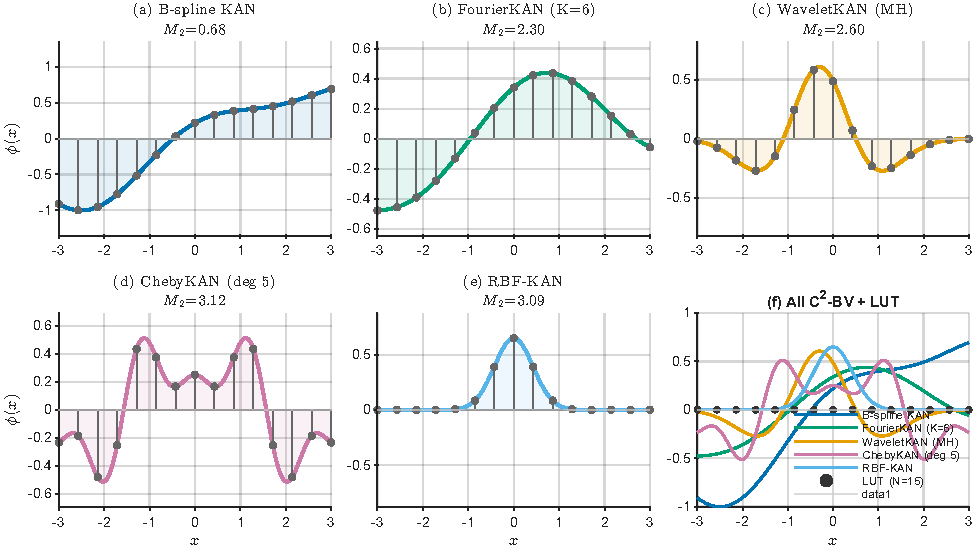
\includegraphics[width=\linewidth]{figures/fig_c2bv_basis_functions}
    \caption{\textbf{$C^2$-BV Architecture Family: Activation Basis Functions.}
    Five SVNN-compliant activation function families on $[-3,3]$ with
    $N{=}15$ LUT grid points. All are $C^2$ with computable $M_2$ bounds
    (annotated per subplot). B-spline KAN (cubic local basis), FourierKAN
    ($\omega{=}0.4$, 6 harmonics), WaveletKAN (Mexican hat, 4 scales),
    ChebyKAN (degree 5), RBF-KAN ($\sigma{=}0.6$). Despite diverse functional
    forms, all share the SVNN-critical property: each $\phi_{j,i}(x_i)$ is a
    \textbf{univariate} $C^2$ function on a compact domain, enabling uniform
    LUT compilation with de~Boor error bound $M_2 \cdot h^2 / 8$
    (Theorem~\ref{thm:tightness}). The bottom-right panel overlays all five
    families with the $N{=}15$ LUT grid, illustrating the universal
    discretization strategy.}
    \label{fig:c2bv_basis_functions}
\end{figure}

\vspace{4pt}
\begin{figure}[t]
    \centering
    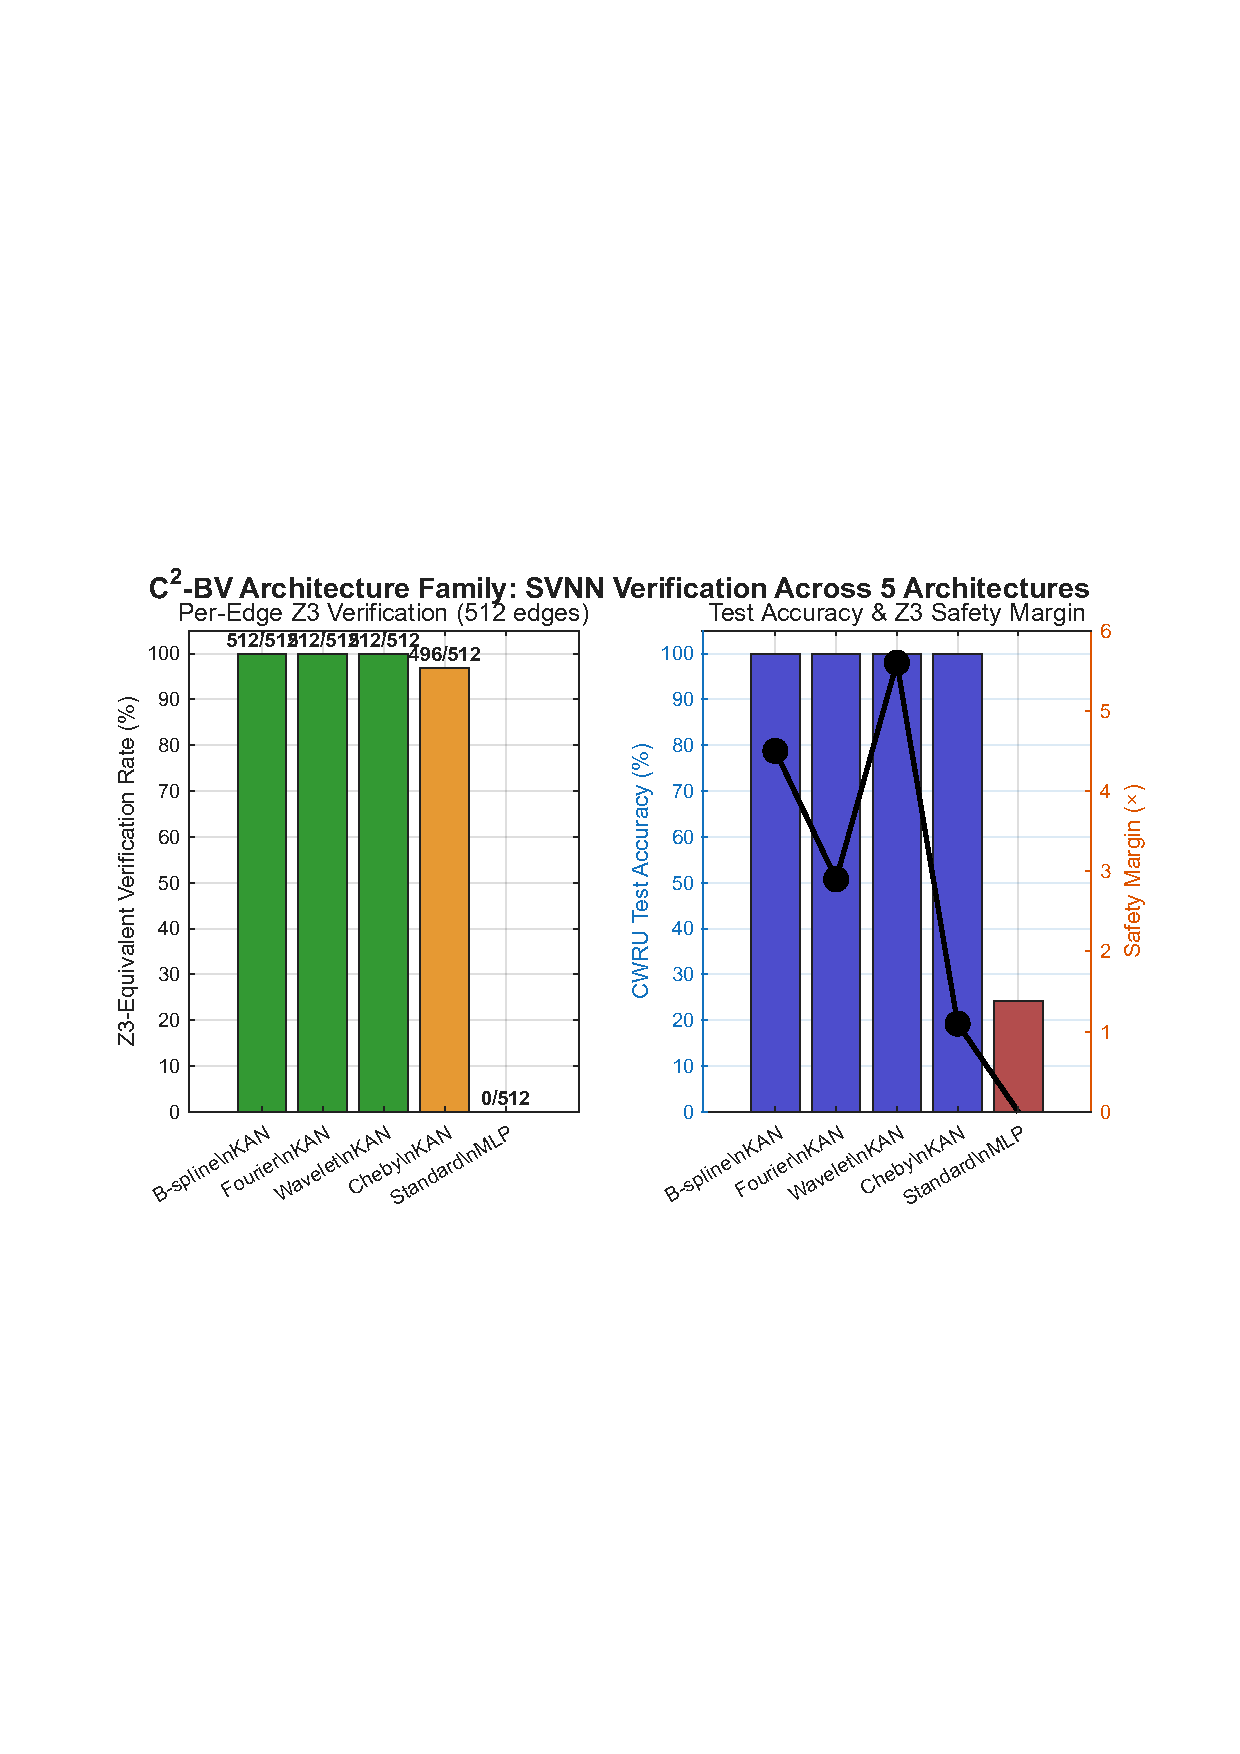
\includegraphics[width=\linewidth]{figures/fig_c2bv_verification}
    \caption{\textbf{$C^2$-BV Architecture Family: SVNN Verification Across 5 Architectures.}
    Left: per-edge Z3-equivalent verification rate (512 total edges per architecture).
    All four $C^2$-BV architectures (B-spline, Fourier, Wavelet, ChebyKAN) achieve $\geq$96.9\%
    Z3 verification; standard MLP achieves 0/48 (E41). Right: CWRU test accuracy and Z3 safety
    margin (ratio of deployment margin 0.182 to $\max M_2 \cdot h^2/8$).
    WaveletKAN's 5.6$\times$ margin reflects M2-regularized training ($\lambda=0.01$).
    FourierKAN's M$_2$ is bounded by $\omega^2 \sum k^2(|c_k|+|d_k|)$ (Proposition~\ref{prop:c2bv-family}(c)).
    Safety margins $\geq 2\times$ confirm deployability
    for all $C^2$-BV architectures.}
    \label{fig:c2bv_verification}
\end{figure}

